% !TeX root = main.tex
\chapter{Measuring audio visualization performance}\label{chp:colourised}

An audio waveform is a plot of the amplitude of an audio signal over time. Waveforms are widely used in audio editing
interfaces as a visual guide to help users navigate the audio. Radio producers interact with audio through the use of
digital audio workstations (DAWs), which display multi-track audio using rows of parallel waveforms. Audio waveforms
are the focal point of these interfaces, and have been since the introduction of DAWs in the early 1980s
\citep{Ingebretsen1982}.

The amplitude profile of a waveform can be used to identify different tracks and see which parts are loud or quiet. It
can be used to identify errors such as clipping and unwanted noise. When viewed at the right resolution, waveforms can
reveal whether the sound is monophonic, polyphonic, tonal or noise-like.  With experience, users can also learn to
map the shape of the waveform to higher-level properties, such as distinguishing music from speech.

In practice, audio recordings are often minutes or hours long. To be able to display these on a screen, only a portion
of the waveform is displayed, which the user controls using pan and zoom commands.  For most practical uses, the
waveform must be zoomed-out to fit on the screen. This reduces the resolution of the waveform in the time dimension,
which means that frequency information and fine variations in the amplitude are no longer visible.  Without frequency
information, users cannot see the pitch, spectrum or timbre of the audio.  This potentially impacts on the ability of
users to efficiently navigate and edit audio content.  Audio waveforms are widely used in audio production software to
help users navigate audio content. The performance of the waveform as a navigational aid is therefore 
important as it affects a large number of users.  However, we were unable to find any studies that have attempted to
measure the effectiveness of waveforms for navigating or editing audio content.

%TODO include this somewhere:
%Audio is often subject to dynamic range compression, which shapes the amplitude profile into a rectangle and further
%impacts on the ability of users to read it.

% waveforms are used in radio production
%The software radio producers use to navigate and edit audio content visualizes the audio using waveforms.
%Many radio producers have been interacting with audio content using waveforms for years, in some cases decades, and in
%that time have learned how the read the waveform to help them with their work.
%However, in Chapter~\ref{chp:background}, we saw that audio waveforms are limited in terms of the information they can
%represent \citep{Rice2005,Loviscach2011,Gohlke2010}.  This potentially impacts on the radio producer's ability to
%navigate and edit their audio content.

%Waveform displays could be enhanced to include additional audio features other than merely the digital signal level.
%The selection of such features and their visual weighting in the display needs to emphasize those possible points of
%interest that reflect the user’s mental model of an audio track and the task at hand. This can include clearly showing
%audio features such as perceptual sample onset, spectrum, timbre, and inaudible issues such as a DC offset.


% the performance of waveforms has not been tested
%Despite their ubiquity, we could not find any studies that have attempted to test how waveforms themselves affect
%interaction with audio.

By designing an audio visualization that can present more information or present it in a way that is robust to zooming,
this may give radio producers a more powerful tool to interact with audio content. We saw in
Chapter~\ref{chp:background} that there have been several previous attempts to create audio visualizations that can
display timbre \citep{Tzanetakis2000,Rice2005}, or assist the navigation of radio broadcasts \citep{Mason2007}.  These
systems worked by extracting semantic audio features and mapping them to a visual representation using pseudocolour or
false colour. Although these systems demonstrated the potential of using enhanced visualizations for aiding navigation
of audio, we could not find any user studies that attempted to measure the impact of this approach.

We were interested in examining how audio visualizations affect audio editing in radio production. In
Section~\ref{sec:vis-method} we describe the design of our user study in which we measured the performance of users in
completing an editing task using different audio visualizations. Section~\ref{sec:vis-results} presents the results,
which show that mapping semantic audio features to colour improved user performance in our task. We discuss what this
might mean for radio production in Section~\ref{sec:vis-discuss}, further work in Section~\ref{sec:vis-further} and
present our conclusions in Section~\ref{sec:vis-conclusions}.

%These techniques could potentially provide applications to radio production and give
%producers better tools for interacting with their content.  However, we could not find any studies that have attempted
%to measure the impact of these visualization techniques on audio production.  As such, we were interested in exploring
%whether semantic audio visualization techniques had an impact on radio production.  To do this, we conducted a study in
%which pariticipants used different audio visualizations to perform a common radio production task, and measured their
%performance.

%\section{Background}

%% WAVEFORM NAVIGATION
%Lots of studies have considered the performance of waveforms for audio navigation, and there are numerous other
%visualizations that perform better.
%However they all use waveforms as the baseline and have not actually measured the performance of the waveform itself.

%% SPEECH/MUSIC DISCRIMINATION
%SMD algorithms all follow the same general approach.
%Raw metric generated, segmented, then clustered.
%Humans are very good at pattern recognition, so by presenting the raw information they may be able to interpret the
%data better than the automated segmenting/clustering.

\section{Methodology}\label{sec:vis-method}

In this study we aimed to evaluate how audio visualizations affect audio editing in radio production.  We designed our
study to measure user performance of a simple task, as this gave us a specific and repeatable action by which we could
assess the effect of different audio visualizations.  We wanted the task to be an activity that is common within radio
production, and to use audio that is representative of that used by radio producers.  However, in order to recruit
enough participants, we wanted to use a task that did not require radio production experience, so that it could be
performed by anybody.

In this section, we describe the task, conditions and audio clips we used for our study. We list the hypotheses we
tested and the metrics we used to do so. We then describe our recruitment process, the design of our test interface,
the protocol of our study and our analysis methodology. 

% The task
\subsection{Task}
For the task, we chose segmentation of music from speech.
In radio production, music has to be removed 
when turning an off-air programme recording into a podcast. This is due to music licensing issues, which are different
for downloadable content than they are for radio broadcasts. The music is removed by editing the audio with a DAW that uses a waveform to
visualize the audio. Although the waveform can be used to distinguish between music and speech, at typical zoom levels
it is not always visible. This means that removing the music can be a slow and tedious process.

% Conditions
\subsection{Conditions}
Radio producers edit audio with DAWs that use audio waveforms for navigating the recordings.  Adding colour to
waveforms would allow us to include additional semantic information about the audio, while being able to retain a
familiar visualization that users are comfortable with and can already read.  Therefore, rather than aiming to replace
the waveform at this stage, we were interested in seeing whether mapping a relevant semantic audio feature to the
colour would impact on the performance of the user's task.

We chose to use the following conditions for the audio visualizations. An example of each condition is shown in
Figure~\ref{fig:conditions}.

\begin{enumerate}[label=C\arabic*.]
  \item \textbf{None}: No visualization, audio only.
  \item \textbf{Waveform}: Audio waveform in a single colour.
  \item \textbf{Enhanced}: Audio waveform with colour mapped to low energy ratio.
\end{enumerate}

\begin{figure}[ht]
  \centering
  \begin{subfigure}{.3\textwidth}
    \centering
    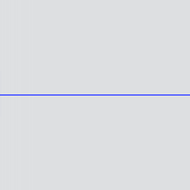
\includegraphics[width=\columnwidth]{figs/condition1.png}
    \caption{C1: None}
  \end{subfigure}
  \begin{subfigure}{.3\textwidth}
    \centering
    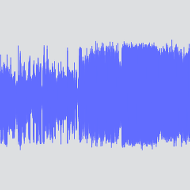
\includegraphics[width=\columnwidth]{figs/condition2.png}
    \caption{C2: Waveform}
  \end{subfigure}
  \begin{subfigure}{.3\textwidth}
    \centering
    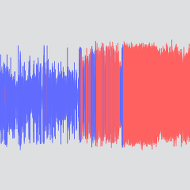
\includegraphics[width=\columnwidth]{figs/condition3.png}
    \caption{C3: Enhanced}
  \end{subfigure}
  \caption{The audio visualization conditions we tested.}
  \label{fig:conditions}
\end{figure}

% Listening
We included a condition in which there was no visualization, as we were interested in using it as a baseline to measure
the performance of the normal waveform. For this condition, the participant must rely purely on listening to the audio.
For the other two conditions, they are able to both listen and use the visualization.

% SMD
For the enhanced visualization, we extracted an audio feature that was relevant to the task and mapped it to the colour
of the waveform.
Speech-music discrimination (SMD) is a research topic that aims to automatically segment speech and music.  This
research often targets recordings of radio broadcasts
\citep{Goodwin2004,Wieser2014,Saunders1996,Pikrakis2008,Pikrakis2006a}. In general, SMD systems extract several audio
features, then use clustering techniques to group those features into segments labelled as either speech or music.
%Clustering is a task in which comes naturally to humans, but machines often struggle with.

% choosing a feature
We wanted to select a feature that would assist the participant in completing their task, but not so much that they
would not have to interpret the information to extract the result. To do this, we restricted ourselves to selecting a
one-dimensional (scalar) feature.
%\citet{Carey1999} found that, other than cepstral features, amplitude-based features performed best.
Low energy ratio (LER, also known as `silent interval frequency', `energy contour dip' and `low short-term energy
ratio') is the frequency in which the energy of a signal falls below a threshold. This is a simple but effective
feature which exploits the fact that speech has frequent silent gaps between words, whereas music does not.
\citet{Panagiotakis2005} found that on its own, LER can classify 50\% of music segments.

% calculating the feature
We calculated the low energy ratio by extracting the RMS energy (20ms frames, no overlap) and counting the proportion
of frames which fell below a threshold.  The threshold can be set as a fixed value \citep{Liang2005,Panagiotakis2005},
a function of the moving average \citep{Ericsson2009}, or a function of the moving peak value \citep{Saunders1996}.
After empirically testing a variety of radio programme recordings, we chose the latter and configured our threshold as
the third percentile of RMS energy in a one second sliding window.

%\[ RMS = \sqrt{\displaystyle\sum\limits_{i=0}^n x_i^2} \]

%Metric does not return perfect results, so user must interpret them

%music tonality \citep{Sell2014}
%energy density analysis \citep{Kacprzak2013}
%??? \citep{Goodwin2004}
%application to TV \citep{Seyerlehner2007}

% mapping the feature
We coloured the waveform by mapping the low energy ratio to a linear gradient between two easily distinguished colours.
We used blue for representing speech, match the waveform colour of the DAW most commonly used in BBC Radio. We used
its inverse colour, pink, to represent music.

\subsection{Audio clips}
We used radio programme recordings for the audio clips, by choosing a representative selection of programme formats,
musical genres and radio stations, shown in Table~\ref{tab:clips}.  We sourced the audio content from `off-air'
recordings of BBC Radio. We selected ten 5-minute clips that contained only one section of music, with speech before
and after. We cut the clips so that the music was in a different position in each clip.  We chose to use nine 5-minute
clips so that the segmentation tasks could be completed in around 15 mins, and one clip for training.

\begin{table}[htbp]
  \begin{center}
    {\small
    \begin{tabular}{l l l l l l}
      \hline
      \textbf{Clip} & \textbf{Network} & \textbf{Prog name} & \textbf{Prog format} & \textbf{Music genre} \\ \hline
      Training & Radio 4 & Desert Island Discs & Interview & Ambient \\
      1 & 1 Xtra & Sian Anderson & Breakfast & Dance \\
      2 & 6 Music & Lauren Laverne & Single & Indie \\
      3 & Radio 2 & Ken Bruce & Phone quiz & Lounge \\
      4 & Radio 3 & Breakfast show & Single & Classical \\
      5 & 5 Live & Sports report & Sports & Band \\
      6 & Radio 1 & Zane Lowe & Interview & Rap \\
      7 & Radio 2 & Jo Whiley & Review & Pop \\
      8 & Radio 4 & Afternoon drama & Drama & Classical \\
      9 & Radio 4 & Front Row & Interview & Alternative \\ \hline
    \end{tabular}
  }
  \end{center}
  \caption{Descriptions of the radio programmes used for the evaluation}
  \label{tab:clips}
\end{table}

\subsection{Hypotheses}

We were interested in testing the effectiveness of audio visualizations for editing audio content. In particular, we
wanted to examine the following hypotheses:

\newcommand{\subscript}[2]{$#1 _ #2$}
\begin{enumerate}[label=H\arabic*.]
  \item \textbf{Effort}: Audio visualization affects the effort required to segment music from speech, in
    decreasing order of C1, C2 and C3.
  \item \textbf{Time}: Audio visualization affects the time taken to segment music from speech, in decreasing
    order of C1, C2 and C3.
  \item \textbf{Accuracy}: Audio visualization affects the accuracy of segmenting music from speech, in
    increasing order of C1, C2 and C3.
    %\item The audio visualization affects the reported task load, in decreasing order of C1, C2 and C3.
\end{enumerate}

\subsection{Metrics}

We measured user performance using quantitative and qualitative metrics.  This allowed us to check for both actual and
perceived differences in performance.

\subsubsection{Quantitative metrics}
Our audio segmentation task involves finding the target audio (in this case, music) and marking the start and end of
the desired region. The two primary activities involved in this are seeking through the audio (by clicking on the
visualization), and marking the segment (using the buttons or sliders). To measure effort, we counted the number of
seek actions (i.e. clicks on the visualization) used to complete the task.

To measure time, we calculated how long it took to complete each task. To avoid including `downtime' at the start and
end of the task, we calculated the task completion time as the difference between the first user action (e.g.
play/seek/mark) and the last marking action.

For accuracy, we measured the error of the result. We calculated this by using ground truth data about the precise
start and end time of the music in the audio, then finding the sum of the absolute error of the selected in-point and
out-point.

\subsubsection{Qualitative metrics}

To gather perceptual data about the tasks, we included a questionnaire for the participants to complete after using
each visualization.  For this, we used the NASA Task Load Index, or `NASA-TLX', \citep{Hart1988} questions, listed
below. Responses are captured using on a scale between -10 and 10 with the following labels at each end.

%\begin{table}[ht]
  %\begin{center}
    %{\small
    %\begin{tabular}{l l l l}
      %\hline
      %Mental demand & How mentally demanding was the task? & very low & very high \\
      %Physical demand & How physically demanding was the task? & very low & very high \\
      %Temporal demand & How hurried or rushed was the pace of the task? & very low & very high \\
      %Performance & How successful were you in accomplishing what you were asked to do? & perfect & failure \\
      %Effort & How hard did you have to work to accomplish your level of performance? & very low & very high \\
      %Frustration & How insecure, discouraged, irritated, stressed, and annoyed were you? & very low & very high \\
      %\hline
    %\end{tabular}
  %}
  %\end{center}
  %\caption{NASA Task Load Index metrics}\
  %\label{tab:nasatlx}
%\end{table}

{\singlespacing
\begin{itemize}
  \item Mental demand -- How mentally demanding was the task? [very low/very high]
  \item Physical demand -- How physically demanding was the task? [very low/very high]
  \item Temporal demand -- How hurried or rushed was the pace of the task?  [very low/very high]
  \item Performance -- How successful were you in accomplishing what you were asked to do? [perfect/failure]
  \item Effort -- How hard did you have to work to accomplish your level of performance? [very low/very high]
  \item Frustration -- How insecure, discouraged, irritated, stressed, and annoyed were you? [very low/very high]
\end{itemize}
}

To measure effort, we used the \textit{effort} rating; to measure time, we used the \textit{temporal demand} rating;
and to measure accuracy, we used the \textit{performance} rating.

We excluding the second part of the NASA-TLX measurement, which converts the sub-scales into a single value by weighting
them by importance \citep{Hart2006}. As such, we are reporting the `Raw TLX' values.  We did this to reduce the time
required for data collection, and to be able to analyse each sub-scale individually.

%{\singlespacing
%\begin{enumerate}
  %\item Waveforms will allow participants to perform speech/music segmentation
  %\begin{enumerate}
    %\item faster
    %\item with less effort
  %\end{enumerate}
  %\item Adding colour to waveforms will allow participants to perform speech/music segmentation
  %\begin{enumerate}
    %\item faster
    %\item with less effort
  %\end{enumerate}
  %\item For speech/music segmentation, participants will rate
  %\begin{enumerate}
   %\item coloured waveforms as easiest to use and least frustrating
   %\item no waveform as hardest to use and most frustrating
  %\end{enumerate}
%\end{enumerate}
%}

\subsection{Recruitment}
We wanted to recruit approximately 50 participants so that our results would have statistical significance.  The radio
production community is relatively small, producers are very busy and they are not used to participating in academic
studies. To get enough respondents, we opted to recruit from a larger pool of technology researchers with experience in
media technology and production.  Additionally, we designed our study so that it could be completed online in 15 mins
or less.  We used email distribution lists to advertise our study to everyone working at BBC Research and Development,
and the Electronics and Computer Science department at Queen Mary University of London.

\subsection{Test interface}
To conduct the experiment, we developed a web-based test interface, shown in Figure~\ref{fig:visualization-interface}.
The interface displayed the overall visualization as well as a zoomed in view above it. The participant could navigate
the audio by clicking on either view, which would seek to that position in the audio.  Buttons below the visualization
controlled play/pause, zoom level and setting the in-- and out-points of the selection.  The selection was displayed by
highlighting the visualization, and on a slider below it. The selection could be adjusted by dragging either end of the
slider.  Training was provided using a `pop-up tour', which guided the user through the interface's features and
operation using a series of pop-up text boxes.  The interface also captured the participant's questionnaire responses
and preferences.  A detailed technical explanation of the interface can be found in
Section~\ref{sec:browser-audio-interface}.

\begin{figure}[ht]
\centering
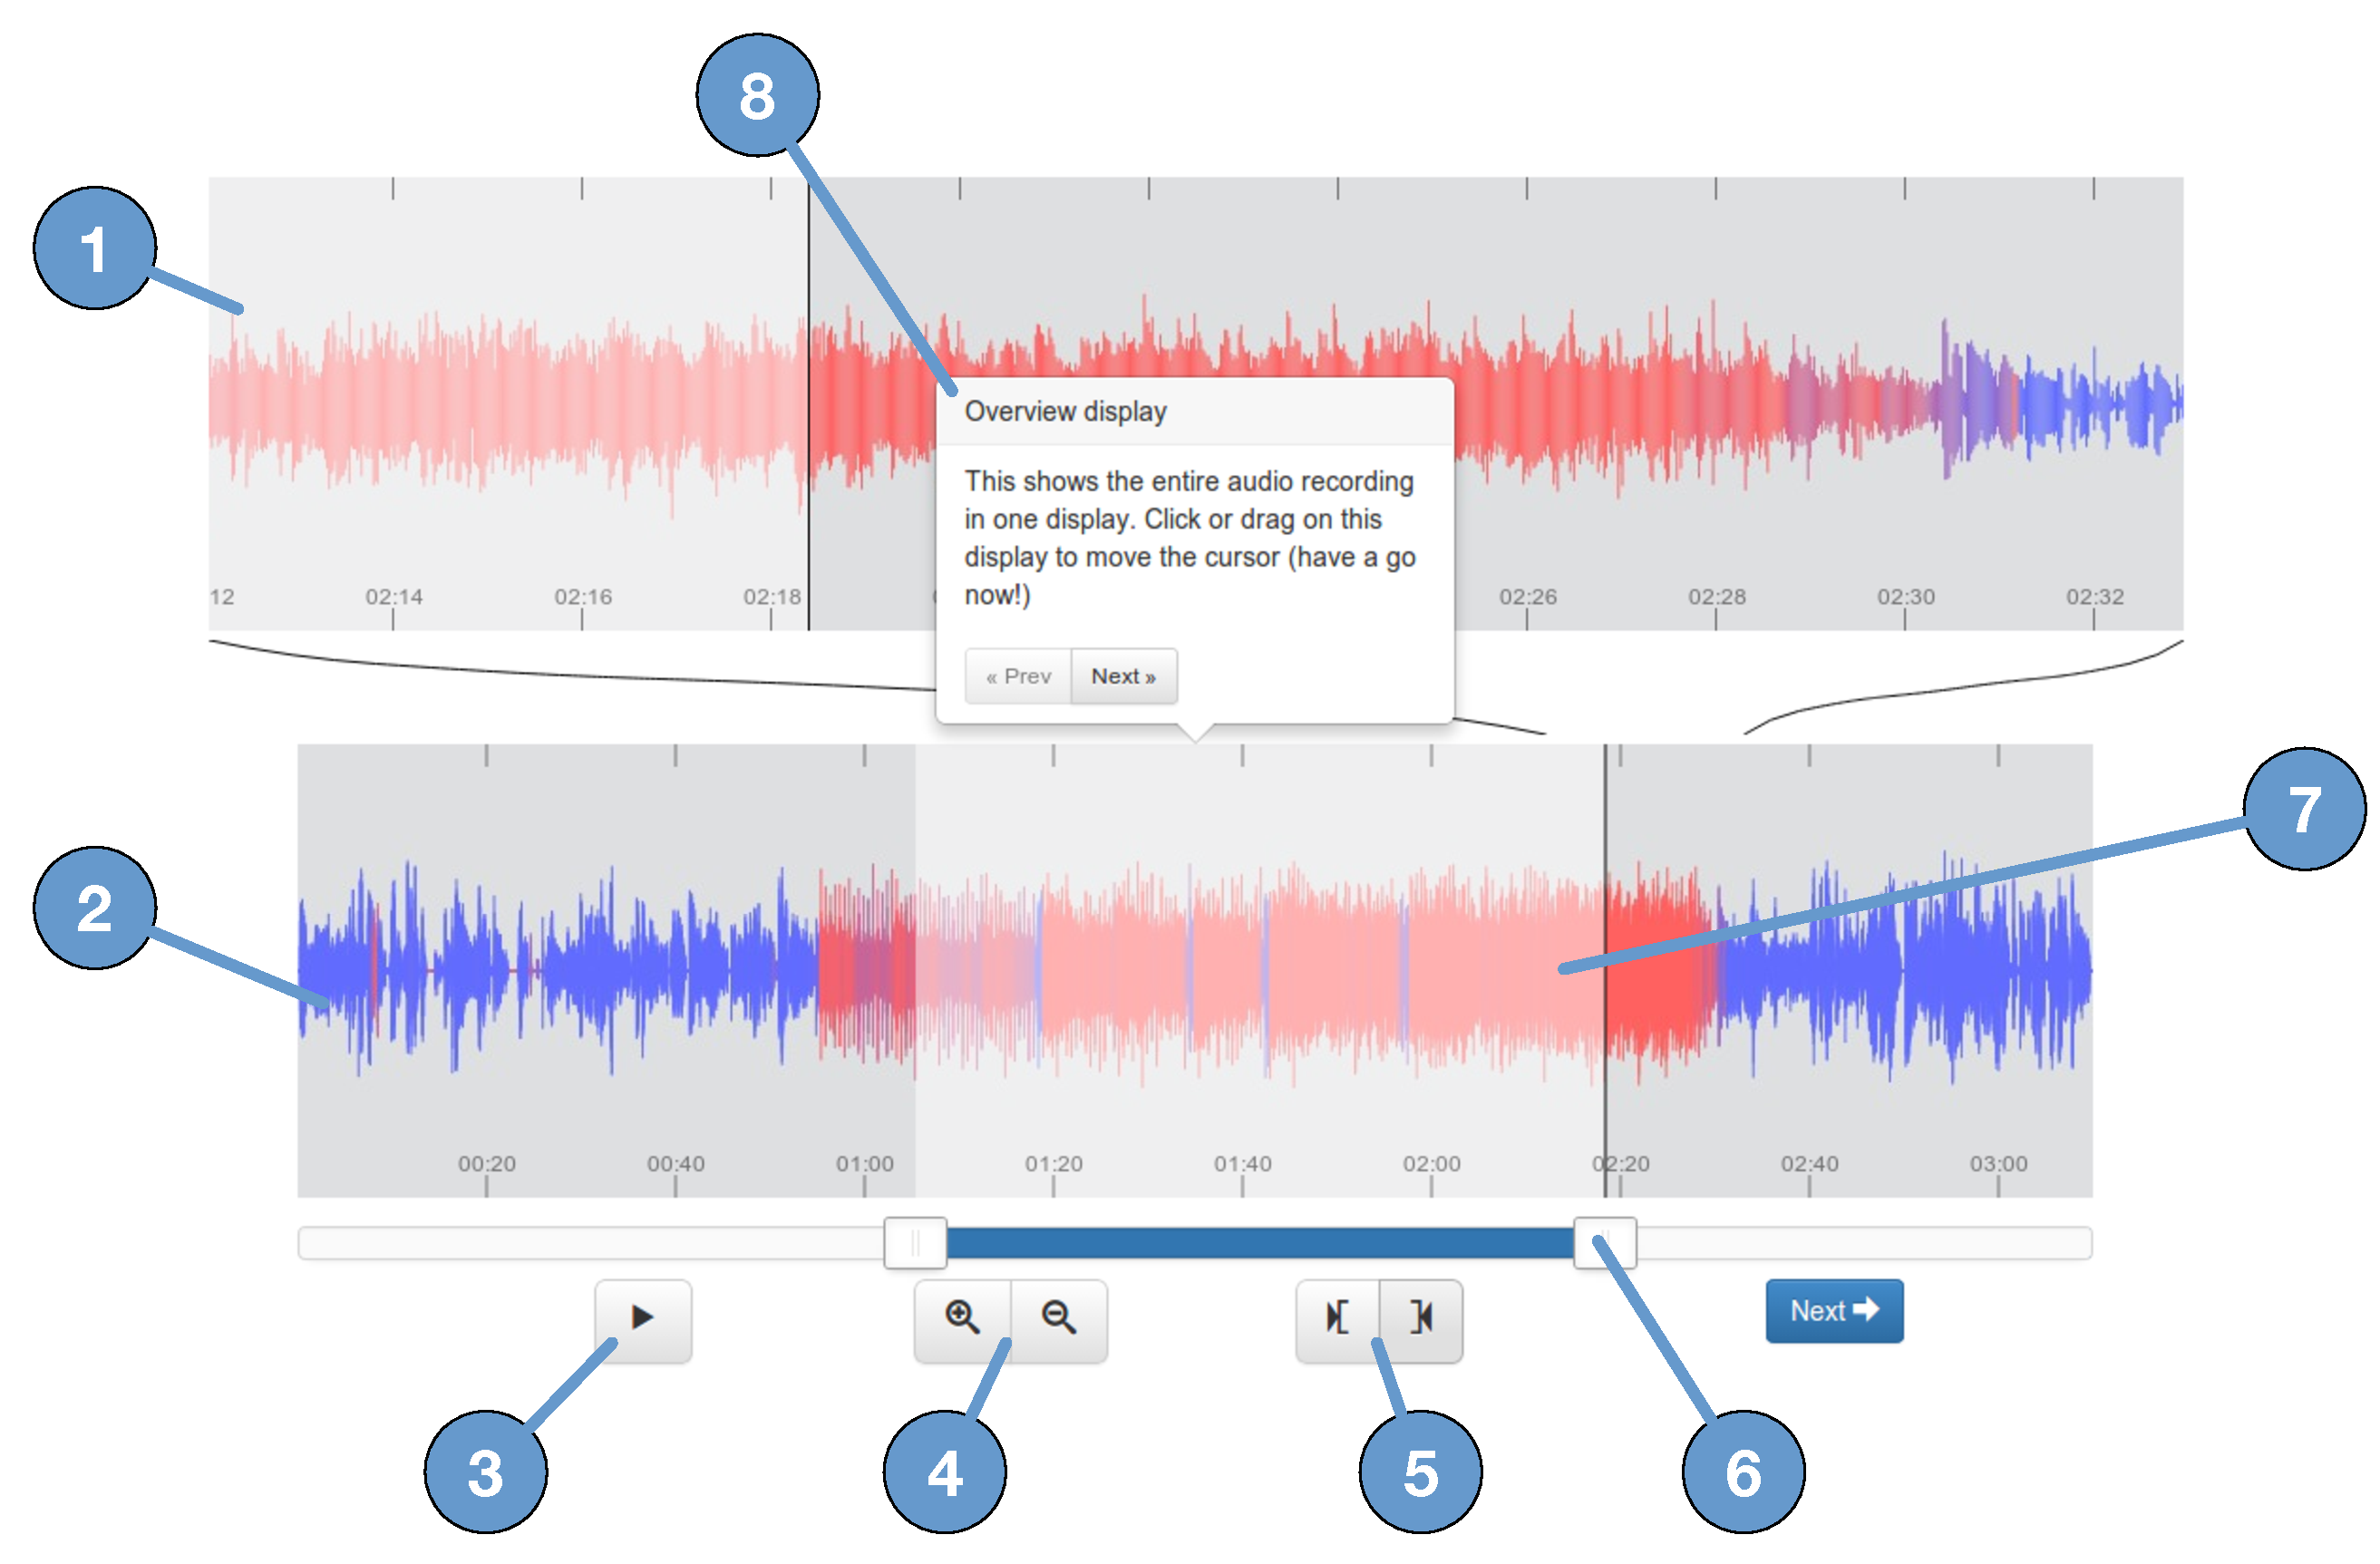
\includegraphics[width=\columnwidth]{figs/browser-audio-interface.pdf}
\caption{Screenshot of the test interface with the following features:
zoomed-in audio visualization (1),
overview audio visualization (2),
play/pause control (3),
zoom in/out control (4),
mark in/out buttons (5),
selection slider (6),
selection highlighting (7),
and training pop-ups (8).}
\label{fig:visualization-interface}
\end{figure}

%We configured the interface to log and timestamp every action the user made, including each seek, play/pause, select
%and zoom action. We also used these metrics to calculate the task completion time, defined as the time between the
%first user action and the last select action.

We generated the visualizations of the audio clips using a plugin framework we developed called `Vampeyer', which
mapped the results of a Vamp audio analysis plugin\footnote{\url{http://www.vamp-plugins.org/}} to a bitmap image. We
then integrated those images into our test interface using in an interactive web-based audio visualization library we
developed called `BeatMap'.  Sections \ref{sec:vampeyer} and \ref{sec:beatmap} contain more detail about Vampeyer and
BeatMap, respectively.

\subsection{Procedure}
Before the study began, we asked the participant to read an information sheet and agree to a consent form. There were
four stages to the study:

\paragraph{Stage 1: Demographics}
We asked the participant about their gender, age and the following questions, to gauge their familiarity with DAWs and
professional experience:

{\singlespacing
\begin{itemize}
  \item Do you understand what an audio waveform is? [Yes/No]
  \item Have you previously used any consumer audio editing software? (e.g.  Audacity, GarageBand) [Yes/No]
  \item Have you previously used any professional audio editing software? (e.g.  ProTools, Logic, Cubase/Nuendo, SADiE,
    Startrack) [Yes/No]
  \item How many years (if any) have you worked with audio in a professional capacity? [\textit{number}]
\end{itemize}
}

\paragraph{Stage 2: Training}
We used a `pop-up tour' to overlay a sequence of text boxes on the interface (see
Figure~\ref{fig:visualization-interface}). These explained the features and operation of the test interface, then
prompted the user to complete and submit a training task. We measured the error of the training task and did not allow
the participant to continue until they had completed the task successfully (defined as an error of less than 5 seconds).

\paragraph{Stage 3: Segmentation task}
The participant used the test interface to mark the position of music in a speech recording, then submit their result.
We logged and timestamped the participant's actions, including seek, play/pause, zoom and mark.  This exercise was
repeated three times for each condition, for a total of nine tasks.  We chose to group the presentation of the
conditions rather than interleave them (e.g. AAABBBCCC instead of ACACBABCB).  We did this so we could capture feedback
directly after each condition, and to avoid possible confusion due to switching too often.

Each audio clip can only be used once per participant, otherwise they would be able to remember the location of the the
music. To define a balanced sequence for the audio clips, we used a Williams design Latin square, generated using the
`crossdes' package\footnote{\url{http://cran.r-project.org/web/packages/crossdes/index.html}} in R.  We used Latin
squares to block out the effect of the order of presentation, and a Williams design, which is balanced for first-order
carryover effects.  As the sequence length is an odd number, the Williams design uses two Latin squares to produce an
$18\times9$ matrix.

To generate the order of visualizations, we needed to produce a balanced $18\times3$ sequence. We did this by taking
three columns from our $18\times9$ Latin square and mapping the values 1--3, 4--6 and 7--9 to 1, 2 and 3, respectively.
By calculating the carryover effect of each column of the $18\times9$ matrix, we found that the middle three columns
had the minimum carryover effect, so we used them for our visualization sequence.

%\begin{table}
%\centering
  %{\small
    %\begin{tabular}{|rrrrrrrrr|}
      %\hline
      %1 & 2 & 9 & 3 & 8 & 4 & 7 & 5 & 6 \\ 
      %3 & 3 & 3 & 2 & 2 & 2 & 1 & 1 & 1 \\ 
      %\hline
      %2 & 3 & 1 & 4 & 9 & 5 & 8 & 6 & 7 \\ 
      %1 & 1 & 1 & 3 & 3 & 3 & 2 & 2 & 2 \\ 
      %\hline
      %3 & 4 & 2 & 5 & 1 & 6 & 9 & 7 & 8 \\ 
      %2 & 2 & 2 & 1 & 1 & 1 & 3 & 3 & 3 \\ 
      %\hline
      %4 & 5 & 3 & 6 & 2 & 7 & 1 & 8 & 9 \\ 
      %3 & 3 & 3 & 2 & 2 & 2 & 1 & 1 & 1 \\ 
      %\hline
      %5 & 6 & 4 & 7 & 3 & 8 & 2 & 9 & 1 \\ 
      %1 & 1 & 1 & 3 & 3 & 3 & 2 & 2 & 2 \\ 
      %\hline
      %6 & 7 & 5 & 8 & 4 & 9 & 3 & 1 & 2 \\ 
      %2 & 2 & 2 & 1 & 1 & 1 & 3 & 3 & 3 \\ 
      %\hline
      %7 & 8 & 6 & 9 & 5 & 1 & 4 & 2 & 3 \\ 
      %3 & 3 & 3 & 2 & 2 & 2 & 1 & 1 & 1 \\ 
      %\hline
      %8 & 9 & 7 & 1 & 6 & 2 & 5 & 3 & 4 \\ 
      %1 & 1 & 1 & 3 & 3 & 3 & 2 & 2 & 2 \\ 
      %\hline
      %9 & 1 & 8 & 2 & 7 & 3 & 6 & 4 & 5 \\ 
      %2 & 2 & 2 & 1 & 1 & 1 & 3 & 3 & 3 \\ 
      %\hline
      %6 & 5 & 7 & 4 & 8 & 3 & 9 & 2 & 1 \\ 
      %1 & 1 & 1 & 2 & 2 & 2 & 3 & 3 & 3 \\ 
      %\hline
      %7 & 6 & 8 & 5 & 9 & 4 & 1 & 3 & 2 \\ 
      %2 & 2 & 2 & 3 & 3 & 3 & 1 & 1 & 1 \\ 
      %\hline
      %8 & 7 & 9 & 6 & 1 & 5 & 2 & 4 & 3 \\ 
      %3 & 3 & 3 & 1 & 1 & 1 & 2 & 2 & 2 \\ 
      %\hline
      %9 & 8 & 1 & 7 & 2 & 6 & 3 & 5 & 4 \\ 
      %1 & 1 & 1 & 2 & 2 & 2 & 3 & 3 & 3 \\ 
      %\hline
      %1 & 9 & 2 & 8 & 3 & 7 & 4 & 6 & 5 \\ 
      %2 & 2 & 2 & 3 & 3 & 3 & 1 & 1 & 1 \\ 
      %\hline
      %2 & 1 & 3 & 9 & 4 & 8 & 5 & 7 & 6 \\ 
      %3 & 3 & 3 & 1 & 1 & 1 & 2 & 2 & 2 \\ 
      %\hline
      %3 & 2 & 4 & 1 & 5 & 9 & 6 & 8 & 7 \\ 
      %1 & 1 & 1 & 2 & 2 & 2 & 3 & 3 & 3 \\ 
      %\hline
      %4 & 3 & 5 & 2 & 6 & 1 & 7 & 9 & 8 \\ 
      %2 & 2 & 2 & 3 & 3 & 3 & 1 & 1 & 1 \\ 
      %\hline
      %5 & 4 & 6 & 3 & 7 & 2 & 8 & 1 & 9 \\ 
      %3 & 3 & 3 & 1 & 1 & 1 & 2 & 2 & 2 \\ 
      %\hline
    %\end{tabular}
    %}
    %\caption{Sequence of presentation of audio clips (top) and visualizations (bottom).}
    %\label{tab:clipseq}
%\end{table}

After completing the three tasks for each condition, the participant rated the workload of those tasks
using the NASA-TLX metrics. We captured the responses using sliders with the labels for each question on either end.

\paragraph{Stage 4: User preference}
After all the tasks were completed, we asked the participant to select which condition they thought was the easiest,
and which was the most frustrating, using the thumbnail images in Figure~\ref{fig:conditions}.

\subsection{Analysis}
We wanted to ensure that all participants completed their tasks correctly.  To do so, we rejected any participant that
submitted a segment with an error of more than five seconds. We calculated the error as the sum of the absolute error
of the in-point and out-point.

%\begin{figure}[ht]
  %\begin{center}
    %$ |t_{in}-t_{inREF}| + |t_{out}-t_{outREF}| \leq 5 $\\[1em]
    %where $t_{in}$ and $t_{out}$ are the in- and out-points of each selection, in seconds,
    %and $t_{inREF}$ and $t_{outREF}$ are the ground truth in- and out-points of the music.
  %\end{center}
  %\caption{Acceptance criteria for the experiment}
  %\label{eq:accept}
%\end{figure}

We tested for statistically significant differences in the task load ratings by using SPSS to conduct a repeated
measures analysis of variance (rANOVA). We then used Tukey's honest significant difference (HSD) post-hoc test to make
pairwise comparisons between the visualization for each metric.

We couldn't re-use audio clips for the tasks, so each participant only experienced a subset of the combinations of
visualizations and audio clips. This resulted in an incomplete dataset, which prevented us from using from using
repeated measures ANOVA. Instead, we used a mixed model as it can account for incomplete data and repeated measures
design.

We used SPSS to perform a linear mixed effects analysis of the relationship between visualization and the three
performance metrics (seek actions, task completion time and task error).  We configured the visualizations as a fixed
effect and the audio clips and participants as random effects.  Visual inspection of residual plots did not reveal any
obvious deviations from homoscedasticity or normality.  We used Fisher's Least Significant Difference (LSD) post-hoc
test to make pairwise comparisons between the visualizations for each metric.

%\paragraph{Box plot}
%A box plot \citep{McGill1978} is a technique used to graph distributions by their quartile values (i.e. 25th, 50th and
%75th percentiles). An example can be seen in Figure~\ref{fig:seekbox}. The box extends from the first to the third
%quartile, with the second quartile (median) marked as a line through the box.  Lines are drawn from the box to the
%minimum and maximum, known as `whiskers', however data determined to be outliers are marked separately as crosses.  The
%95\% confidence interval of the median is marked as a notch in the box.

%\paragraph{ANOVA}
%Analysis of variance is a method of testing whether the mean values of several groups are equal or not. It assumes that
%the observations are independent, that the data have a normal distribution, and that the variance within the groups are
%similar. One-way ANOVA tests for a null hypothesis that the means values of the factors are the same.

%\paragraph{Tukey's test}
%If the null hypothesis is rejected using ANOVA, we know that there is a difference between the factors, but we don't
%know which ones. Tukey's test is a post-hoc analysis for discovering the difference between individual factors.  It
%assumes that the observations are independent and that the variance within the groups are similar.

%When Tukey's test is graphed, the mean values are represented by a dot with a line either side showing the confidence
%interval. Confidence intervals which don't overlap can be said to be significantly different.

%\paragraph{Standardisation}
%Some observations can be biased through participant behaviour. For example, person A navigates audio recordings by
%quickly clicking along the timeline while person B navigates with only a few considered clicks. To block this factor,
%the responses of each participant can be standardised so that they have a mean value of 0 and a standard deviation of
%1. This allows the difference between different participants responses to be measured fairly.

%Standardisation maps observations to the `\textbf{standard score}'. This is a dimensionless unit which represents the
%number of standard deviations an observation is above the mean.

\section{Results}\label{sec:vis-results}
63 participants completed the study. Of those, 41 (65\%) passed the acceptance criteria. This was lower than expected,
so we analysed the rejected tasks and participants to look for evidence of any systematic errors that might explain the
high number of rejections.

\begin{figure}[h]
\centering
  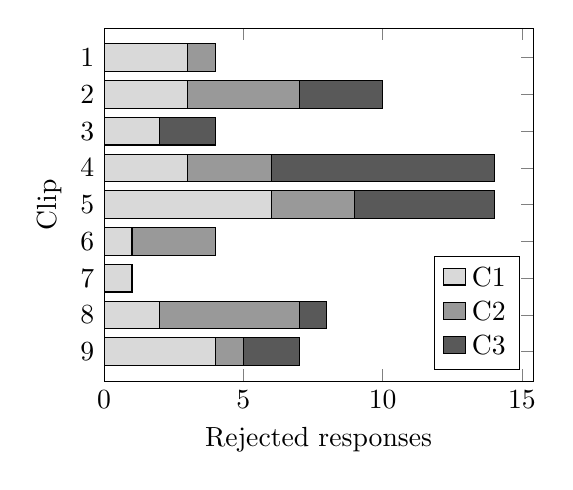
\begin{tikzpicture}
    \begin{axis}[
      height=0.5\textwidth,
      %width=0.9\textwidth,
      legend pos=south east,
      legend cell align=left,
      xbar stacked,
      ytick=data,
      xmin=0,
      ylabel=Clip,
      xlabel=Rejected responses,
      symbolic y coords={9,8,7,6,5,4,3,2,1},
    ]
    \addplot[fill=black!15] coordinates
      {(4,9) (2,8) (1,7) (1,6) (6,5) (3,4) (2,3) (3,2) (3,1)};
    \addplot[fill=black!40] coordinates
      {(1,9) (5,8) (0,7) (3,6) (3,5) (3,4) (0,3) (4,2) (1,1)};
    \addplot[fill=black!65] coordinates
      {(2,9) (1,8) (0,7) (0,6) (5,5) (8,4) (2,3) (3,2) (0,1)};
    \legend{C1,C2,C3}
    \end{axis}
  \end{tikzpicture}
  \caption{Rejected clips}
  \label{fig:rejected-clips}
\end{figure}

Figure~\ref{fig:rejected-clips} shows the number of clips and conditions that were used for the rejected responses.
Although clips 4 and 5 had a higher number of rejections, the incorrect responses came from all clips and all
conditions. There was also no combination of clips and conditions that caused an unusually high number of rejections.
We did not find any notable difference in error between the in-points and out-points.  Figure~\ref{fig:demographics}
shows the demographics of the participants.  We did not find any correlation between rejected participants and DAW
experience, professional experience, age or gender.

\begin{figure}[h]
\centering
\begin{subfigure}{.5\textwidth}
  \centering
  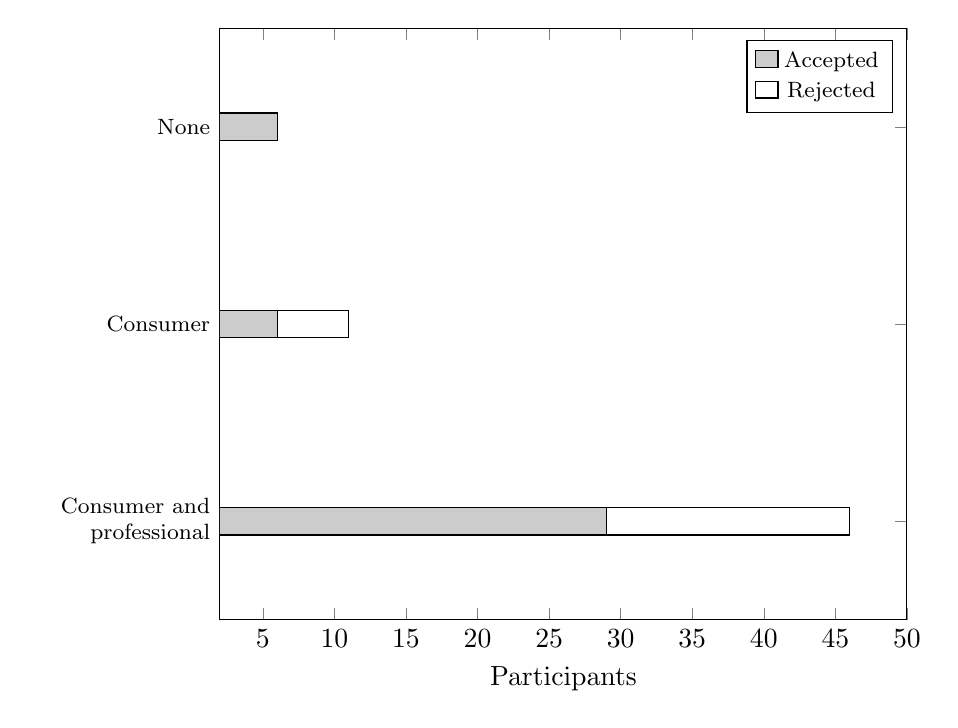
\begin{tikzpicture}
    \begin{axis}[
      height=0.75\textwidth,
      width=0.85\textwidth,
      enlarge y limits=0.25,
      xbar stacked,
      ytick=data,
      yticklabel style={font=\footnotesize,text width=2.2cm,align=right},
      xlabel=Participants,
      symbolic y coords={Consumer and professional,Consumer,None},
      legend style={font=\footnotesize},
    ]
    \addplot[fill=black!20] coordinates
      {(29,Consumer and professional) (6,Consumer) (6,None)};
    \addplot[fill=white] coordinates
      {(17,Consumer and professional) (5,Consumer) (0,None)};
    \legend{Accepted,Rejected}
    \end{axis}
  \end{tikzpicture}
  \caption{DAW experience}
  \label{fig:daw-experience}
\end{subfigure}%
\begin{subfigure}{.5\textwidth}
  \centering
  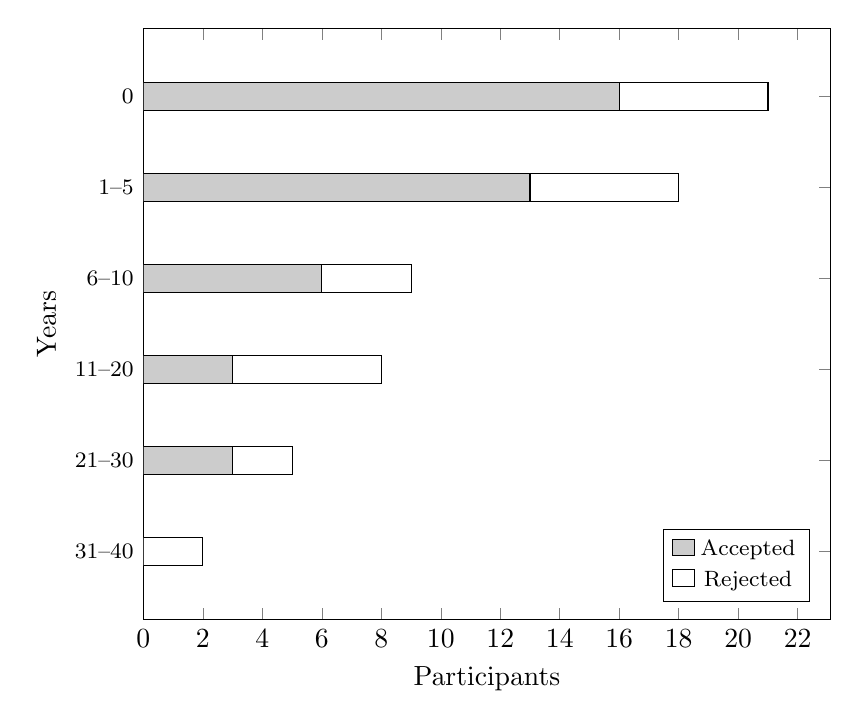
\begin{tikzpicture}
    \begin{axis}[
      height=0.75\textwidth,
      width=0.85\textwidth,
      legend pos=south east,
      enlarge y limits=0.15,
      xbar stacked,
      ytick=data,
      yticklabel style={font=\footnotesize},
      xmin=0,
      ylabel=Years,
      xlabel=Participants,
      symbolic y coords={31--40,21--30,11--20,6--10,1--5,0},
      legend style={font=\footnotesize},
    ]
    \addplot[fill=black!20] coordinates
      {(0,31--40) (3,21--30) (3,11--20) (6,6--10) (13,1--5) (16,0)};
    \addplot[fill=white] coordinates
      {(2,31--40) (2,21--30) (5,11--20) (3,6--10) (5,1--5) (5,0)};
    \legend{Accepted,Rejected}
    \end{axis}
  \end{tikzpicture}
  \caption{Professional experience}
  \label{fig:pro-experience}
\end{subfigure}
\caption{Participant demographics}
\label{fig:demographics}
\end{figure}

We were unable to find any systematic errors that would explain the rejected responses. However, as the test was online
and unsupervised, this may have led some participants to perform the task to a lower standard than was required.

Figure~\ref{fig:demographics} shows that the vast majority of participants had previous experience of using both
consumer and professional audio editing software. 61\% of participants also had professional experience of working with
audio. All participants reported that they understood what an audio waveform was.
%The demographic of the participants showed a heavy bias (80\%) of male participants, and a larger proportion in the
%26-45 age range (see Figure~\ref{fig:age}). This reflects the population to which the experiment was promoted (see
%Section~\ref{sec:promo}) and is not expected to skew the results.


%\begin{figure}[ht]
  %\centering
  %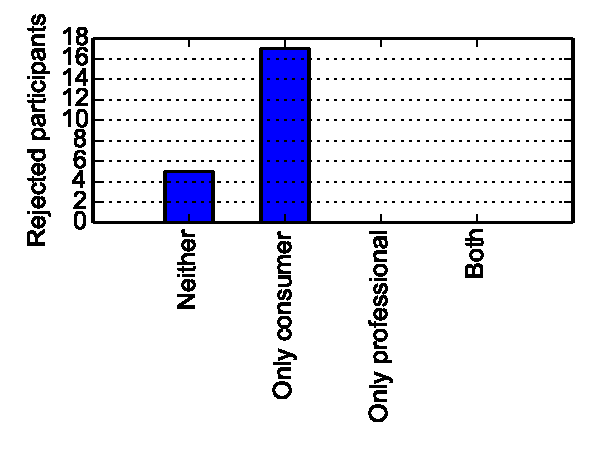
\includegraphics[width=0.5\textwidth]{figs/reject-daw.pdf}
  %\caption{Response of rejected participants when asked whether they had previously used consumer/professional audio
    %editing software}
  %\label{fig:rejectdaw}
%\end{figure}

%\begin{figure}[ht]
%\centering
%\begin{subfigure}{.5\textwidth}
  %\centering
  %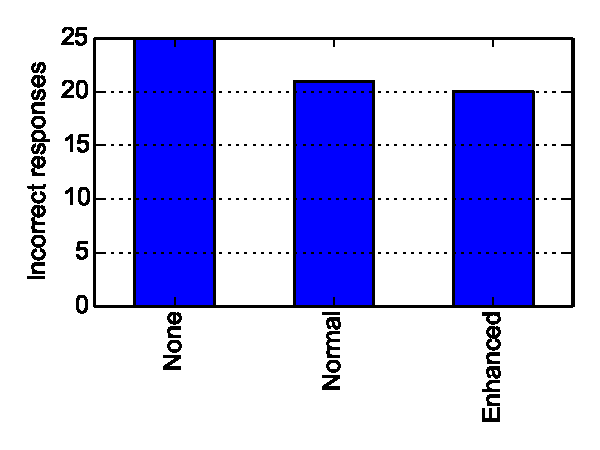
\includegraphics[width=\linewidth]{figs/rejects-vis.pdf}
  %\caption{By visualization}
  %\label{fig:rejectvis}
%\end{subfigure}%
%\begin{subfigure}{.5\textwidth}
  %\centering
  %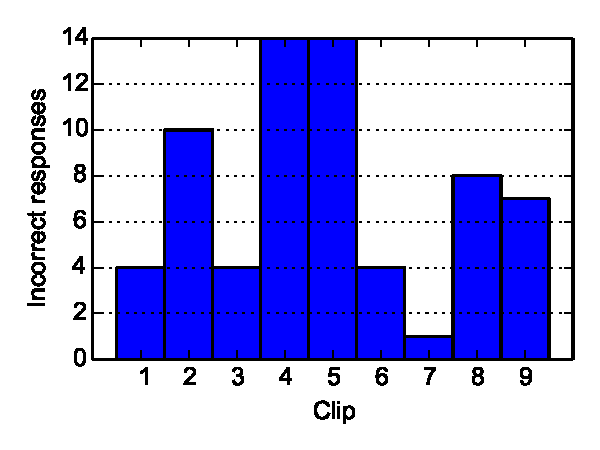
\includegraphics[width=\linewidth]{figs/rejects-clip.pdf}
  %\caption{By clip}
  %\label{fig:rejectclip}
%\end{subfigure}
%\caption{Analysis of incorrect responses}
%\label{fig:rejects}
%\end{figure}

%\begin{figure}[ht]
  %\centering
  %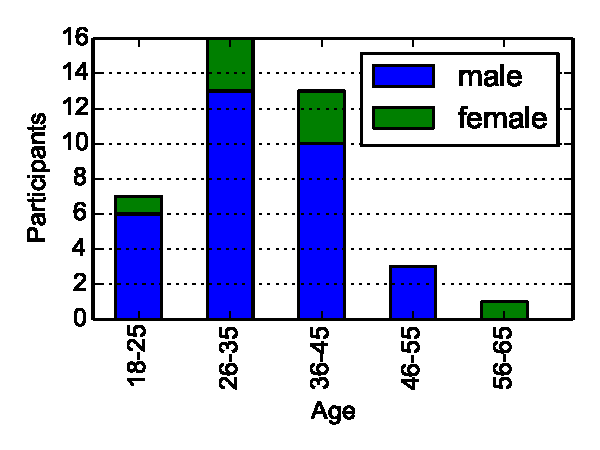
\includegraphics[width=0.5\textwidth]{figs/age.pdf}
  %\caption{Age and gender of participants. Male/female ratio was 32/8
    %(80\%/20\%). One participant declined to respond to the question.}
  %\label{fig:age}
%\end{figure}

%\begin{figure}[ht]
%\centering
%\begin{subfigure}{.5\textwidth}
  %\centering
  %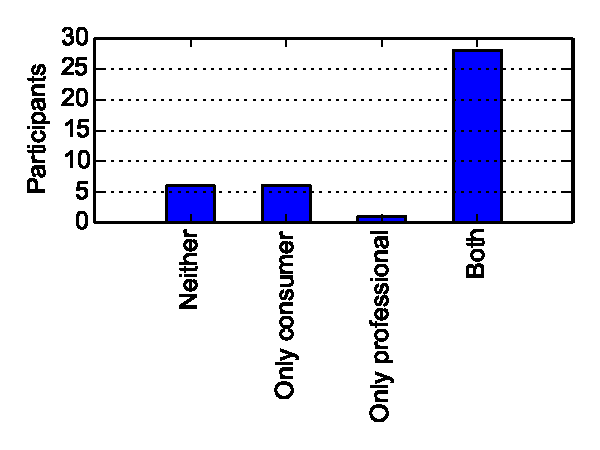
\includegraphics[width=\textwidth]{figs/daw.pdf}
  %\caption{Previous use of audio editing software}
  %\label{fig:experiencedaw}
%\end{subfigure}%
%\begin{subfigure}{.5\textwidth}
  %\centering
  %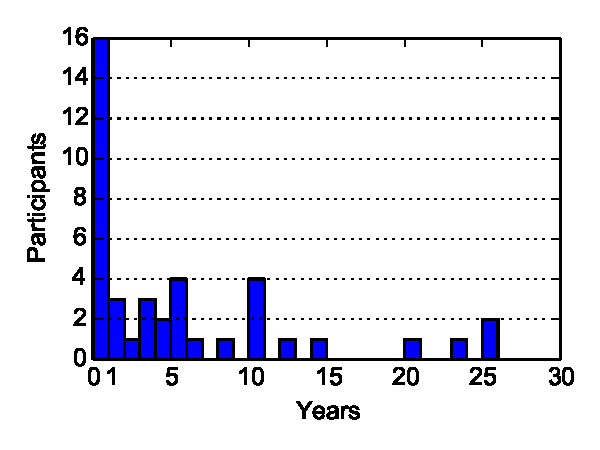
\includegraphics[width=\linewidth]{figs/experience.pdf}
  %\caption{Years of professional audio experience}
  %\label{fig:experienceyears}
%\end{subfigure}
%\caption{Response of participants to questions about experience}
%\label{fig:experience}
%\end{figure}

\subsection{Quantitative metrics}

We analysed the quantitative performance metrics using a linear mixed model.
%Our model found statistically significant differences
%between the three conditions for seek actions, task time, and task error.
Figure~\ref{fig:visualization-metrics} shows
the mean values and confidence intervals of the performance metrics and Table~\ref{tab:pairwise-performance} lists the
statistical significance of the pairwise comparisons between the conditions.

\begin{figure}[ht]
  \centering
  \begin{subfigure}[t]{0.5\textwidth}
    \centering
    \begin{tikzpicture} 
    \begin{axis}[
      width=\textwidth,
      ylabel=count,
      xtick={1,2,3},
      xticklabels={C1,C2,C3}]
      \addplot[black,mark=*]
        plot[error bars/.cd, y dir=both, y explicit]
        coordinates {
          (1, 29.5) +- (3.7,3.7)
          (2, 24.3) +- (3.6,3.6)
          (3, 16.8) +- (3.1,3.1)
        };
    \end{axis} 
    \end{tikzpicture}
    \caption{Seek actions}
  \end{subfigure}%
  ~
  \begin{subfigure}[t]{0.5\textwidth}
    \centering
    \begin{tikzpicture} 
    \begin{axis}[
      width=\textwidth,
      ylabel=seconds,
      xtick={1,2,3},
      xticklabels={C1,C2,C3}]
      \addplot[black,mark=*]
        plot[error bars/.cd, y dir=both, y explicit]
        coordinates {
          (1, 0.645) +- (0.121,0.121)
          (2, 0.610) +- (0.121,0.121)
          (3, 0.523) +- (0.109,0.109)
        };
    \end{axis} 
    \end{tikzpicture}
    \caption{Task error}
  \end{subfigure}

  \begin{subfigure}[t]{0.5\textwidth}
    \centering
    \begin{tikzpicture} 
    \begin{axis}[
      width=\textwidth,
      ylabel=seconds,
      xtick={1,2,3},
      xticklabels={C1,C2,C3}]
      \addplot[black,mark=*]
        plot[error bars/.cd, y dir=both, y explicit]
        coordinates {
          (1, 70.6) +- (16.76,16.76)
          (2, 68.7) +- (16.49,16.49)
          (3, 59.7) +- (16.47,16.47)
        };
    \end{axis} 
    \end{tikzpicture}
    \caption{Task completion time}
  \end{subfigure}
  \caption{Mean performance metric values with 95\% confidence intervals. Lower values are better.}
  \label{fig:visualization-metrics}
\end{figure}

\definecolor{lightred}{RGB}{255,204,204}
\definecolor{lightamber}{RGB}{255,204,153}
\definecolor{lightgreen}{RGB}{204,255,204}
\newcommand{\highsig}{\cellcolor{black!20}}
\newcommand{\medsig}{\cellcolor{black!10}}
\newcommand{\nosig}{\cellcolor{white}}
\begin{table}[ht]
    \begin{tabular}{L{.35\textwidth-2\tabcolsep} C{.21\textwidth-2\tabcolsep} C{.21\textwidth-2\tabcolsep} C{.23\textwidth-2\tabcolsep}}
\hline
& \textbf{C1 vs C2} & \textbf{C2 vs C3} & \textbf{C1 vs C3} \\ \hline
	Seek actions        & \highsig$<0.01$ & \highsig$<0.01$ & \highsig$<0.01$ \\
	Task completion time& \nosig$>0.05$   & \highsig$<0.01$ & \highsig$<0.01$ \\
	Task error          & \nosig$>0.05$   & \medsig$<0.05$  & \highsig$<0.01$  \\
\end{tabular}
\caption{$p$-values of pairwise comparisons for the performance metrics. Statistically significant differences are shaded.}
\label{tab:pairwise-performance}
\end{table}


\subsubsection{Seek actions}
The audio visualization had a significant effect on the number of seek actions used to complete the task
[$F(3,366)=93.871, p<.00001$]. Based on the mean averages, the enhanced waveform (C3) required 7.5 (30\%) fewer seek
actions than the normal waveform (C2), and 12.7 (43\%) fewer than having no visualization (C1). Additionally, the
normal waveform (C2) required 5.2 (17\%) fewer seek actions than having no visualization (C1).  The differences in seek
actions between all three conditions were statistically significant ($p<.01$). These results confirm hypothesis H1
(effort).

\subsubsection{Task completion time}
The audio visualization had a significant effect on the time required to complete the task [$F(3,366)=25.261,
p<.00001$].  Based on the mean averages, the task was completed 9 seconds (13\%) faster using the enhanced waveform
(C3) compared to the normal waveform (C2), and 10.9 seconds (15\%) faster compared to having no
visualization (C1), both with $p<.01$.  There was no statistically significant difference in task completion time between the
normal waveform (C2) and no visualization (C1).  The mean time of the normal waveform was only 1.9 seconds (3\%) faster
than no visualization.  These results suggest that hypothesis H2 (time) is confirmed for C2$>$C3, but not for C1$>$C2.

\subsubsection{Task error}
The audio visualization had a significant effect on the accuracy of the task result [$F(3,366)=42.462, p<.00001$].
Based on the mean averages, the error when using the enhanced waveform (C3) was 87ms (14\%) lower than when using the
normal waveform (C2) with $p<.05$, and 122ms (19\%) lower than when there was no visualization (C1) with $p<.01$. There
was no statistically significant difference in task error between the normal waveform (C2) and no visualization (C1).
The error using the normal waveform was only 35ms (5\%) less than with no visualization.  These results suggest that
hypothesis H3 (accuracy) is confirmed for C2$<$C3, but not for C1$<$C2.

%\begin{figure}[ht] \centering \begin{subfigure}{.5\textwidth} \centering
%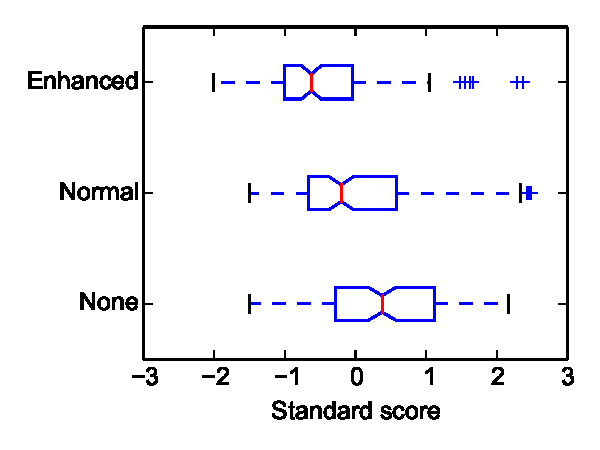
\includegraphics[width=\textwidth]{figs/seek-std.pdf} \caption{Box plot} \label{fig:seekbox} \end{subfigure}%
%\begin{subfigure}{.5\textwidth} \centering 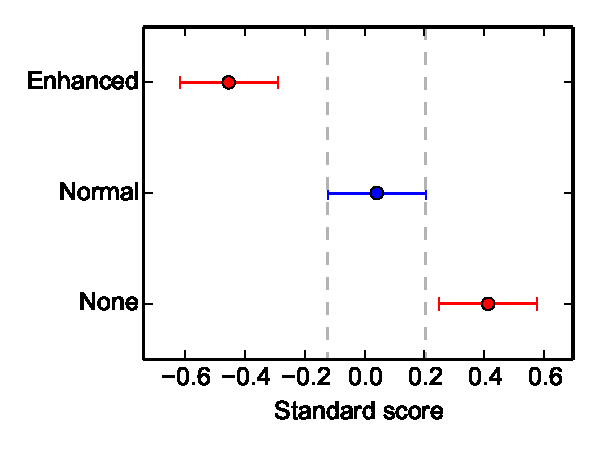
\includegraphics[width=\linewidth]{figs/seek-std-tukey99.pdf}
%\caption{Tukey's test (99\% confidence interval)} \label{fig:seektukey} \end{subfigure} \caption{Number of seek
%actions, standardised per participant} \label{fig:seek} \end{figure}

%\begin{figure}[ht] \centering \begin{subfigure}{.5\textwidth} \centering
%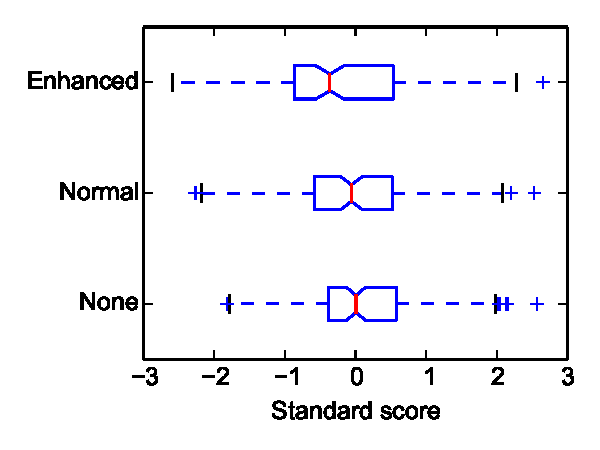
\includegraphics[width=\textwidth]{figs/playstart-to-selectend-std.pdf} \caption{Box plot} \label{fig:selecttimebox}
%\end{subfigure}% \begin{subfigure}{.5\textwidth} \centering
%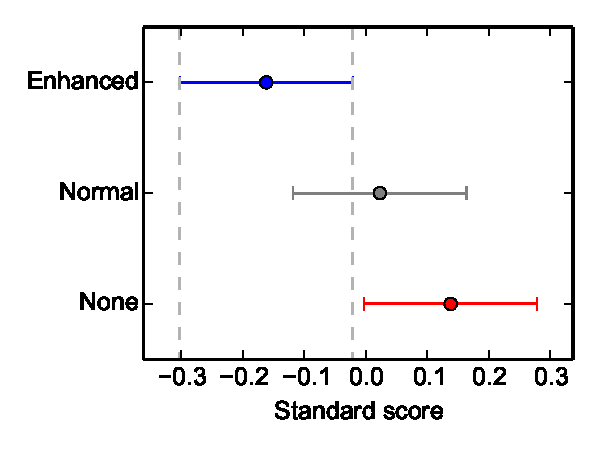
\includegraphics[width=\linewidth]{figs/playstart-to-selectend-std-tukey95.pdf} \caption{Tukey's test (95\% confidence
%interval)} \label{fig:selecttimetukey} \end{subfigure} \caption{Selection time (time between start of playback and
%final selection), standardised per participant} \label{fig:selecttime} \end{figure}

%\begin{figure}[ht]
%\centering
%\begin{subfigure}{.5\textwidth}
  %\centering
  %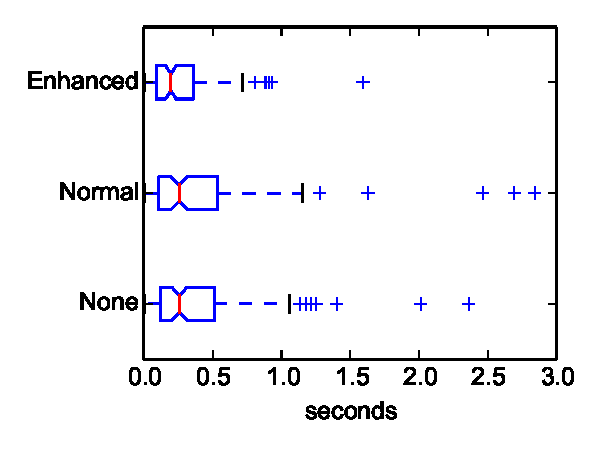
\includegraphics[width=\textwidth]{figs/outpoint-abserr.pdf}
  %\caption{Box plot}
  %\label{fig:outpointerrbox}
%\end{subfigure}%
%\begin{subfigure}{.5\textwidth}
  %\centering
  %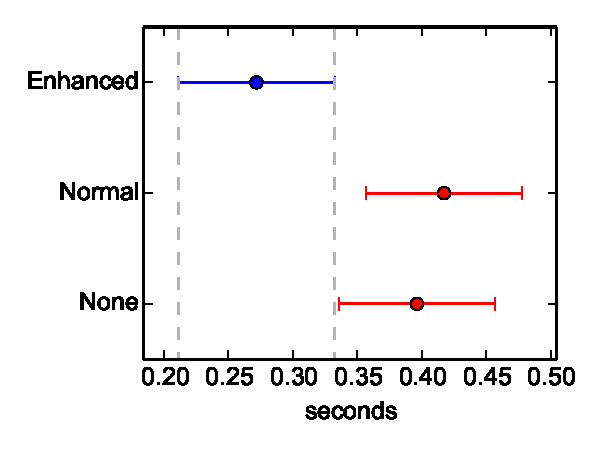
\includegraphics[width=\linewidth]{figs/outpoint-abserr-tukey95.pdf}
  %\caption{Tukey's test (95\% confidence interval)}
  %\label{fig:outpointerrtukey}
%\end{subfigure}
%\caption{Absolute error for the outpoint of selections}
%\label{fig:outpointerr}
%\end{figure}

%\paragraph{Zoom}
%The experimental interface included two displays -- one overview display covering the length of the recording, and a
%zoomed display which showed a magnified part of that. The number of times the zoom in and zoom out buttons were pressed
%was logged. The sum of these values for each visualization is shown in Figure~\ref{fig:zoomtotal}. By subtracting zoom
%out from zoom in, we can infer what the final zoom level was when the response was submitted. The final zoom levels for
%each visualization are shown in Figure~\ref{fig:zoomfinal}.

%\begin{figure}[h!]
%\centering
%\begin{subfigure}{.5\textwidth}
  %\centering
  %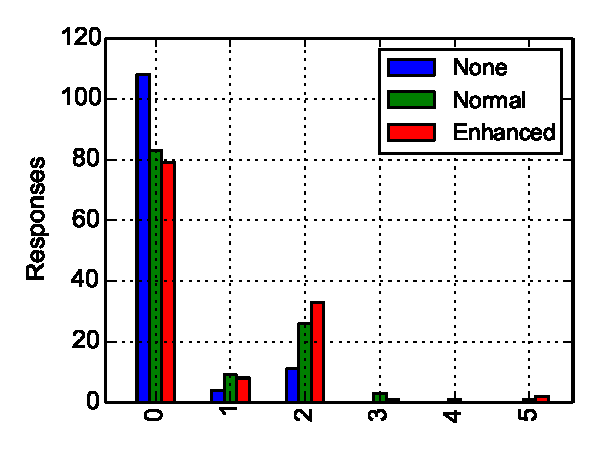
\includegraphics[width=\linewidth]{figs/zoomtotal.pdf}
  %\caption{Total zoom actions}
  %\label{fig:zoomtotal}
%\end{subfigure}%
%\begin{subfigure}{.5\textwidth}
  %\centering
  %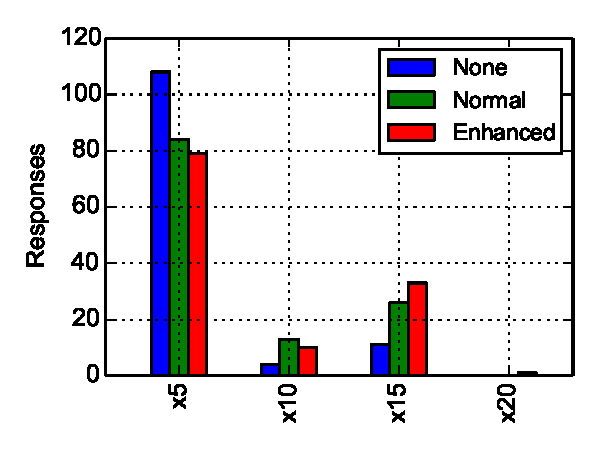
\includegraphics[width=\linewidth]{figs/zoomfinal.pdf}
  %\caption{Final zoom level}
  %\label{fig:zoomfinal}
%\end{subfigure}
%\caption{Analysis of zoom usage}
%\label{fig:zoom}
%\end{figure}

%Most of the time, participants didn't touch the zoom controls and opted to leave it on the default x5 zoom level, which
%displays roughly one minute of audio across 1045 pixels ($\sim$50ms per pixel). Other than the x5 level, x15 was more
%popular than x10 for all visualizations and x20 was barely used at all.

\subsection{Qualitative metrics}

We analysed the task load ratings using repeated measures multivariate ANOVA, which found that the audio visualization
had a significant effect on the task load ratings from participants [$F(12,152)=3.552, p<0.001$].
Figure~\ref{fig:tlx-results} shows the mean values and confidence intervals of the task load metrics and
Table~\ref{tab:pairwise-perceptual} lists the statistical significance of the pairwise comparisons between the conditions.

\begin{table}[ht]
  \begin{threeparttable}
    \begin{tabular}{L{.35\textwidth-2\tabcolsep} C{.21\textwidth-2\tabcolsep} C{.21\textwidth-2\tabcolsep} C{.23\textwidth-2\tabcolsep}}
\hline
& \textbf{C1 vs C2} & \textbf{C2 vs C3} & \textbf{C1 vs C3} \\ \hline
  Effort\tnote{1} & \medsig$<0.05$  & \highsig$<0.01$ & \highsig$<0.01$ \\
	Frustration     & \medsig$<0.05$  & \medsig$<0.05$  & \highsig$<0.01$  \\
	Mental demand   & \nosig$>0.05$   & \highsig$<0.01$ & \highsig$<0.01$ \\
	Performance     & \nosig$>0.05$   & \medsig$<0.05$  & \highsig$<0.01$  \\
	Physical demand & \nosig$>0.05$   & \highsig$<0.01$ & \highsig$<0.01$ \\
  Temporal demand\tnote{1} & \nosig$>0.05$ & \medsig$<0.05$ & \nosig$>0.05$ \\ \hline
\end{tabular}
\caption{$p$-values of pairwise comparisons for the perceptual metrics. Statistically significant differences are shaded.}
\label{tab:pairwise-perceptual}
\begin{tablenotes}
    \item[1] Mauchly's Test of Sphericity indicated that the assumption of sphericity had been violated for the effort
      metric [$\chi^2(2) = 9.657, p=.008$] and temporal demand metric [$\chi^2(2) = 17.918, p<.001$]. Therefore, we
      have adjusted the degrees of freedom for the univariate tests using the conservative Greenhouse-Geisser
      Correction.
  \end{tablenotes}
  \end{threeparttable}
\end{table}

The task load ratings from participants show that compared to both the normal waveform (C2) and no visualization (C1),
the enhanced waveform (C3) was less mentally and physically demanding, had better performance, was less frustrating and
required less effort (all $p<0.05$).  They also rated the enhanced waveform as less temporally demanding than the normal
waveform ($p<0.05$).  Compared to having no visualization (C1), participants rated the normal waveform (C2) as being
less frustrating and requiring less effort (both $p<0.05$). 

The effort ratings confirm hypothesis H1 (effort); the temporal demand ratings confirm hypothesis H2 (time) for
C2$>$C3; and the performance ratings confirm hypothesis H3 (accuracy) for C2$<$C3.

\begin{figure}[p]
  \centering
  \begin{subfigure}[t]{0.5\textwidth}
    \centering
    \begin{tikzpicture} 
    \begin{axis}[
      width=\textwidth,
      ylabel=Effort,
      xtick={1,2,3},
      xticklabels={C1,C2,C3}]
      \addplot[black,mark=*]
        plot[error bars/.cd, y dir=both, y explicit]
        coordinates {
          (1, -0.122) +- (1.49,1.49)
          (2, -2.244) +- (1.51,1.51)
          (3, -4.220) +- (1.28,1.28)
        };
    \end{axis} 
    \end{tikzpicture}
    \caption{Effort}
  \end{subfigure}%
  ~
  \begin{subfigure}[t]{0.5\textwidth}
    \centering
    \begin{tikzpicture} 
    \begin{axis}[
      width=\textwidth,
      ylabel=Frustration,
      xtick={1,2,3},
      xticklabels={C1,C2,C3}]
      \addplot[black,mark=*]
        plot[error bars/.cd, y dir=both, y explicit]
        coordinates {
          (1, -0.829) +- (2.03,2.03)
          (2, -2.976) +- (1.67,1.67)
          (3, -5.268) +- (1.24,1.24)
        };
    \end{axis} 
    \end{tikzpicture}
    \caption{Frustration}
  \end{subfigure}%

  \begin{subfigure}[t]{0.5\textwidth}
    \centering
    \begin{tikzpicture} 
    \begin{axis}[
      width=\textwidth,
      ylabel=Mental demand,
      xtick={1,2,3},
      xticklabels={C1,C2,C3}]
      \addplot[black,mark=*]
        plot[error bars/.cd, y dir=both, y explicit]
        coordinates {
          (1, -1.390) +- (1.68,1.68)
          (2, -2.585) +- (1.45,1.45)
          (3, -4.585) +- (1.23,1.23)
        };
    \end{axis} 
    \end{tikzpicture}
    \caption{Mental demand}
  \end{subfigure}%
  ~
  \begin{subfigure}[t]{0.5\textwidth}
    \centering
    \begin{tikzpicture} 
    \begin{axis}[
      width=\textwidth,
      ylabel=Performance,
      xtick={1,2,3},
      xticklabels={C1,C2,C3}]
      \addplot[black,mark=*]
        plot[error bars/.cd, y dir=both, y explicit]
        coordinates {
          (1, -5.415) +- (1.10,1.10)
          (2, -6.317) +- (1.11,1.11)
          (3, -7.341) +- (0.88,0.88)
        };
    \end{axis} 
    \end{tikzpicture}
    \caption{Performance}
  \end{subfigure}%

  \begin{subfigure}[t]{0.5\textwidth}
    \centering
    \begin{tikzpicture} 
    \begin{axis}[
      width=\textwidth,
      ylabel=Physical demand,
      xtick={1,2,3},
      xticklabels={C1,C2,C3}]
      \addplot[black,mark=*]
        plot[error bars/.cd, y dir=both, y explicit]
        coordinates {
          (1, -3.122) +- (1.81,1.81)
          (2, -4.098) +- (1.45,1.45)
          (3, -6.171) +- (1.08,1.08)
        };
    \end{axis} 
    \end{tikzpicture}
    \caption{Physical demand}
  \end{subfigure}%
  ~
  \begin{subfigure}[t]{0.5\textwidth}
    \centering
    \begin{tikzpicture} 
    \begin{axis}[
      width=\textwidth,
      ylabel=Temporal demand,
      xtick={1,2,3},
      xticklabels={C1,C2,C3}]
      \addplot[black,mark=*]
        plot[error bars/.cd, y dir=both, y explicit]
        coordinates {
          (1, -3.171) +- (1.75,1.75)
          (2, -3.268) +- (1.51,1.51)
          (3, -4.878) +- (1.39,1.39)
        };
    \end{axis} 
    \end{tikzpicture}
    \caption{Temporal demand}
  \end{subfigure}%
  \caption{Mean NASA-TLX values with 95\% confidence intervals. Lower values are better.}
  \label{fig:tlx-results}
\end{figure}

%\begin{figure}[p]
  %\centering
  %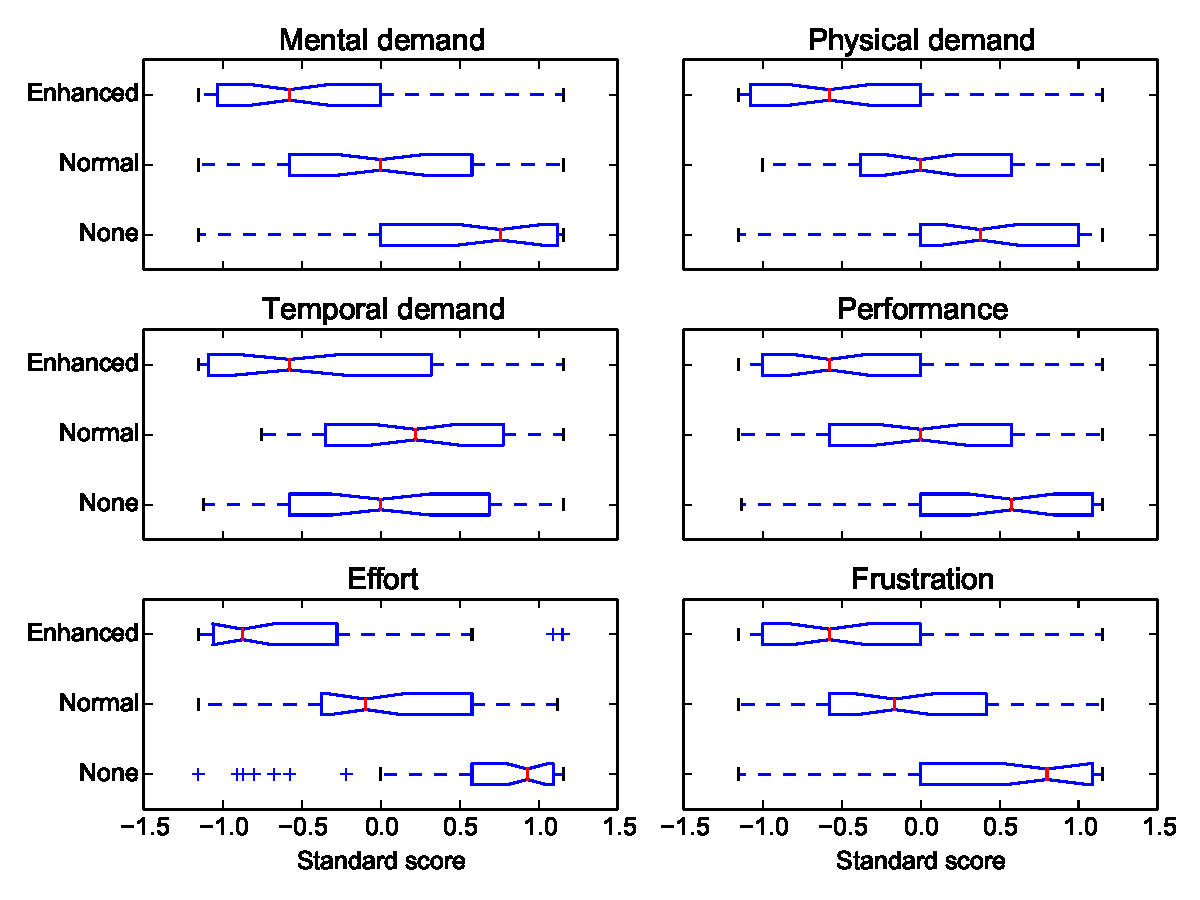
\includegraphics[width=\textwidth]{figs/tlx-std.pdf}
  %\caption{Standard score of NASA Task Load Index responses for each visualization, standardised per participant.}
  %\label{fig:tlx}
%\end{figure}

%\begin{figure}[p]
  %\centering
  %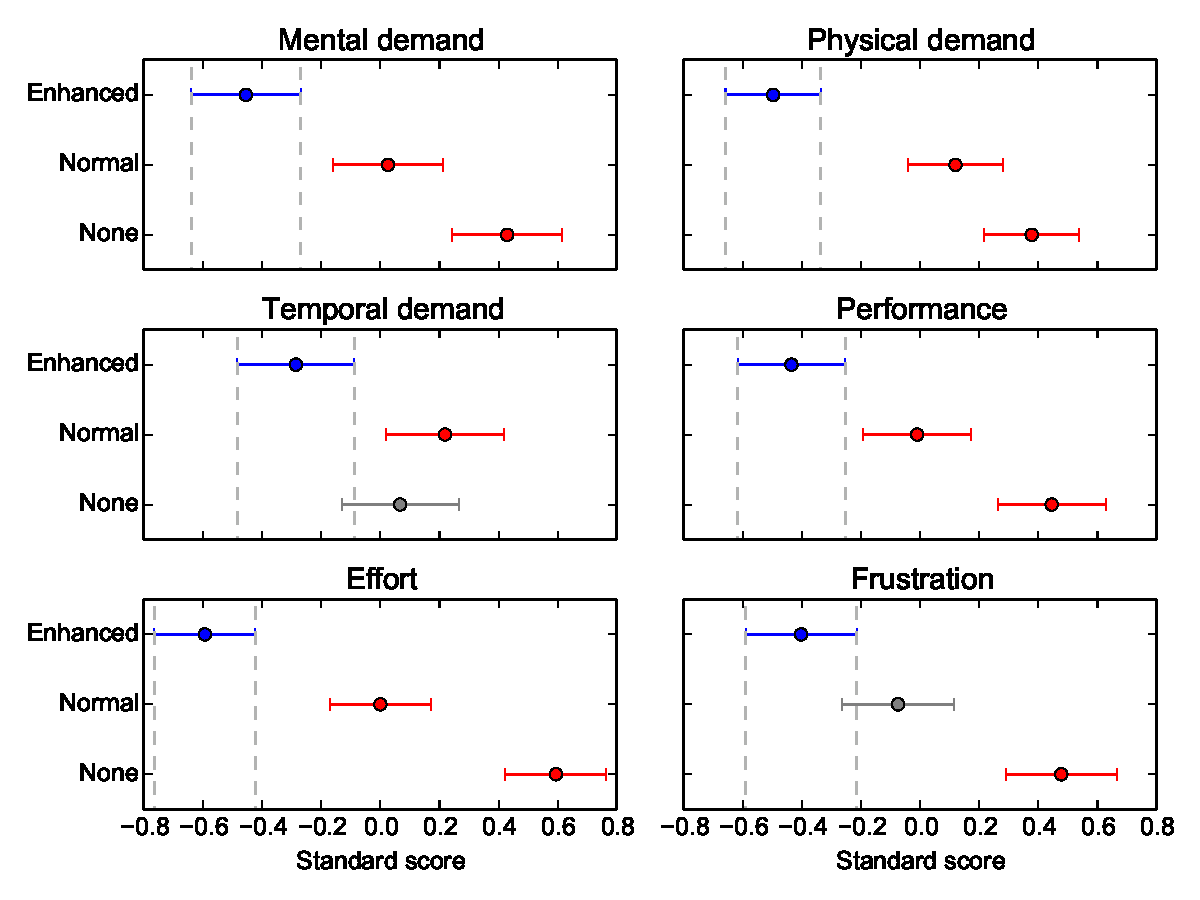
\includegraphics[width=\textwidth]{figs/tlx-std-tukey95.pdf}
  %\caption{Standard score of NASA Task Load Index responses for each visualization, standardised per participant.}
  %\label{fig:tlxtukey}
%\end{figure}

The participants rated the enhanced waveform (C3) as significantly less physically demanding than the normal waveform
(C2).  This was surprising, as all of the tasks were conducted using a screen and mouse, so did not require much
physical exertion.  We do not know how participants interpreted this metric, but it's possible that some may have
classified the movement of the mouse or number of mouse clicks as physical activity.

Participants were asked to select which audio visualization was the easiest to use, and which was the most frustrating.
The results are shown in Figure~\ref{fig:visualization-comparison}.  The enhanced waveform (C3) was rated as the
easiest to use by 76\% of the participants.  Having no visualization (C1) was rated as the most frustrating condition
by two-thirds of the participants. The normal waveform (C2) was not considered by many to be the easiest, nor the most
frustrating.

\begin{figure}[ht]
\centering
\begin{subfigure}{.5\textwidth}
  \centering
  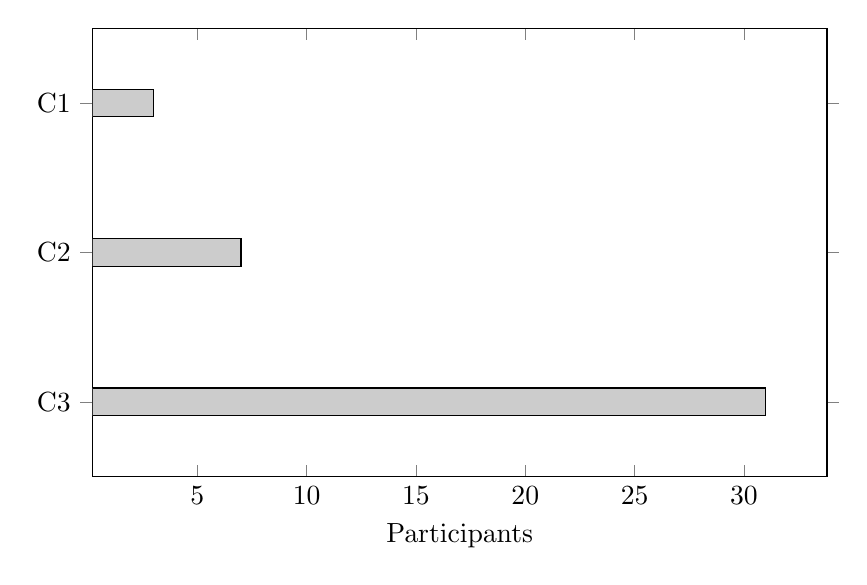
\begin{tikzpicture}
    \begin{axis}[
      height=0.6\textwidth,
      width=0.9\textwidth,
      %xmin=0,
      %xmax=38,
      enlarge y limits=0.25,
      xbar,
      ytick=data,
      xlabel=Participants,
      symbolic y coords={C3,C2,C1},
      %nodes near coords, nodes near coords align={horizontal},
    ]
    \addplot[fill=black!20] coordinates
      {(31,C3) (7,C2) (3,C1)};
    \end{axis}
  \end{tikzpicture}
  \caption{Easiest}
  \label{fig:easiest}
\end{subfigure}%
\begin{subfigure}{.5\textwidth}
  \centering
  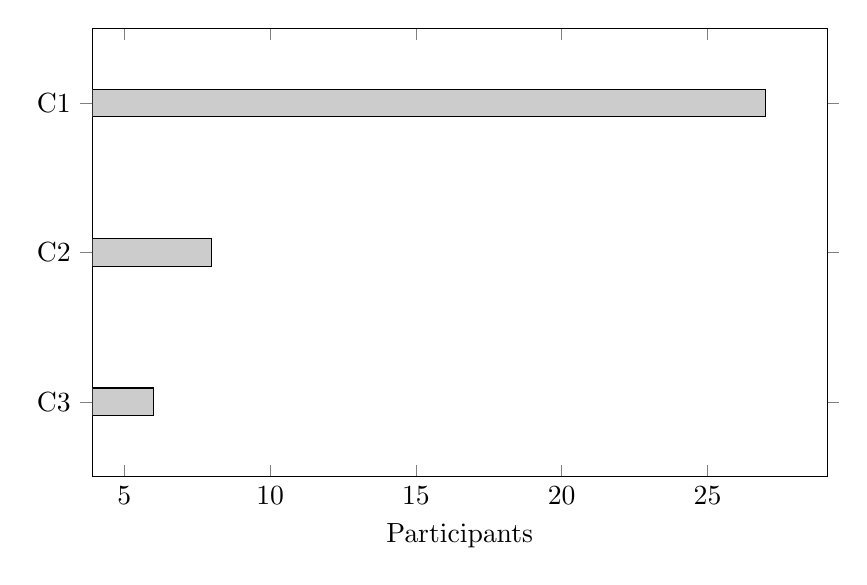
\begin{tikzpicture}
    \begin{axis}[
      height=0.6\textwidth,
      width=0.9\textwidth,
      %xmin=0,
      %xmax=32,
      enlarge y limits=0.25,
      xbar,
      ytick=data,
      xlabel=Participants,
      symbolic y coords={C3,C2,C1},
      %nodes near coords, nodes near coords align={horizontal},
    ]
    \addplot[fill=black!20] coordinates
      {(6,C3) (8,C2) (27,C1)};
    \end{axis}
  \end{tikzpicture}
  \caption{Most frustrating}
  \label{fig:frustrating}
\end{subfigure}
\caption{Preferences of participants}
\label{fig:visualization-comparison}
\end{figure}


%\begin{figure}[ht]
%\centering
%\begin{subfigure}{.5\textwidth}
  %\centering
  %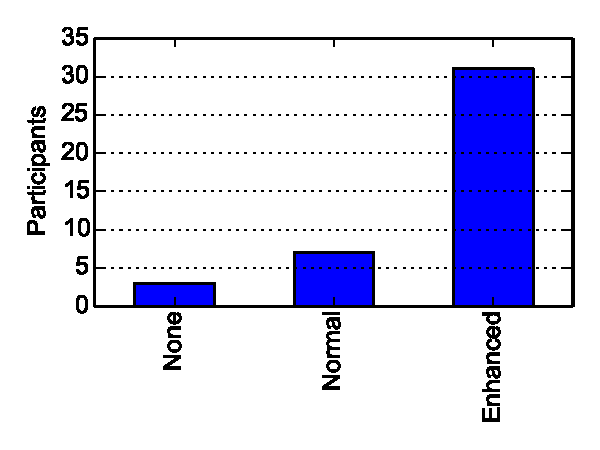
\includegraphics[width=\textwidth]{figs/easiest.pdf}
  %\caption{Easiest to use}
  %\label{fig:easiest}
%\end{subfigure}%
%\begin{subfigure}{.5\textwidth}
  %\centering
  %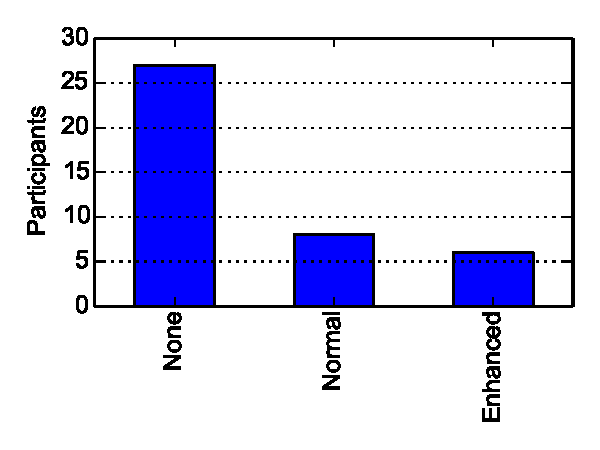
\includegraphics[width=\linewidth]{figs/frustrating.pdf}
  %\caption{Most frustrating}
  %\label{fig:frustrating}
%\end{subfigure}
%\caption{Response of participants when asked to compare the visualizations
  %using different criteria}
%\label{fig:compare}
%\end{figure}

%\subsection{Interaction behaviour}
%This section looks at how participants used the features available in the online audio interface, full described in
%Section~\ref{sec:iface}.
%Informal observation of some participants as they completed the experiment
%revealed that some people used the interface in different ways. For example,
%when one participant had completed their selection, they scanned through the
%remaining unselected content to check that there were no other pieces of music.

%\begin{figure}[ht]
%\centering
%\begin{subfigure}{.5\textwidth}
  %\centering
  %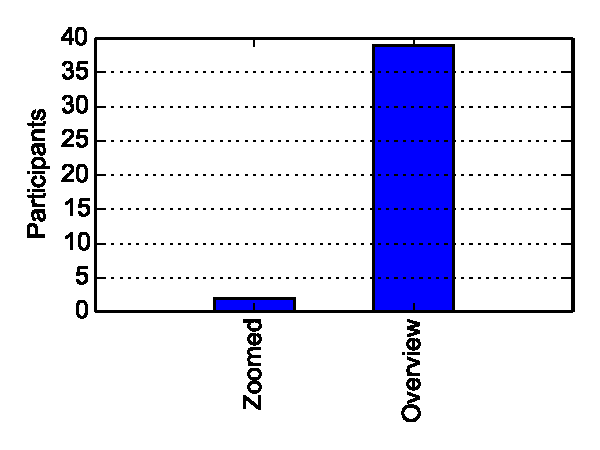
\includegraphics[width=\linewidth]{figs/top-v-bot-pref.pdf}
  %\caption{Display}
  %\label{fig:displaypref}
%\end{subfigure}%
%\begin{subfigure}{.5\textwidth}
  %\centering
  %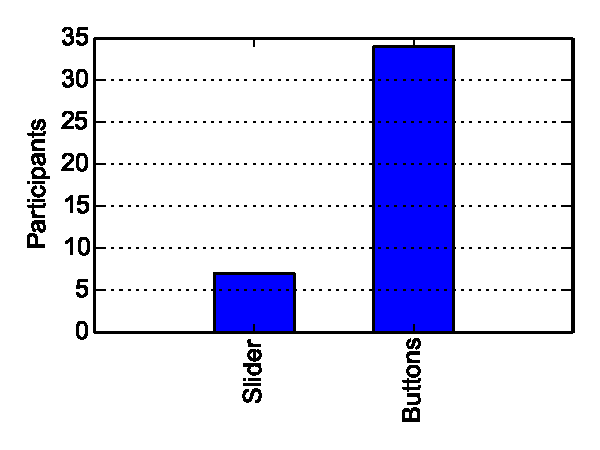
\includegraphics[width=\linewidth]{figs/mark-v-slide-pref.pdf}
  %\caption{Selection method}
  %\label{fig:selectpref}
%\end{subfigure}
%\caption{Preference of participants}
%\label{fig:pref}
%\end{figure}

%\paragraph{Top/bottom display}
%There are two displays that make up the interface -- a zoomed display at the top and an overview display on the bottom.
%Either of the displays can be used to navigate the recording and make selections.

%For each participant, the number of tasks where they used the zoom display more than the overview (and vice-versa) were
%counted. Figure~\ref{fig:displaypref} shows number of participants who, on average, used the zoomed or overview display
%more.

%The results show a clear preference for using the overview display more than the zoom display. Coupled with the results
%of zoom usage in Section~\ref{sec:studymetrics}, we can see that for this task most people opted just to work in the
%overview display, despite only having a resolution of roughly 300ms per pixel.

%An analysis of the overview and zoom display's usage between different visualization methods did not find any notable
%difference.

%\paragraph{Selection method}
%The design of the interface gave participants two methods of making a selection -- buttons to mark in and out points
%using the cursor, and a slider where the in and out points could be dragged around. The cursor can be moved around in
%both the overview and zoomed displays, whereas the slider is only available at the x1 zoom level. This makes the
%buttons more useful for fine edits, where high precision is needed. When using the slider, the selection display
%updates as you move it making it easier for people to see where their selection is.

%For each response, the method with the most actions was found and these preferences were summed for each participant to
%calculate their overall preference. The results are shown in Figure~\ref{fig:selectpref}.

%The buttons were the most popular method of making a selection, with only 17\% of people using the slider more.
%Informal feedback found that some people has a strong preference for using the slider but were frustrated that there
%wasn't a second slider available on the zoomed display.

%\section{Results}
%63 responses were received in the three weeks the experiment ran. 35\% of participants were rejected, which was higher
%than expected. An analysis of the rejected participants found that none had experience of using professional audio
%editing software, which suggests that the errors could be due to lack of experience with audio interfaces.

%The demographic of accepted participants reflected the population which was recruited: 80\% male with a larger
%proportion in the 26-45 age range. This imbalance is not expected to affect the result. Two-thirds of accepted
%participants had experience of using professional audio editing software, with the remaining participants having
%consumer-level experience or less. 39\% reported having no professional experience with audio.

%Figure~\ref{fig:seekpdf} shows the distribution of the number of seek actions for each visualization. On average, the
%number of seek actions required to select the music is lowest for the enhanced waveform and highest for no waveform.
%However, individual participants had different styles of interaction; for example, some people had a tendency to seek
%around a lot whereas others didn't. In order to account for this, the performance and TLX metrics were standardised for
%each participant.

%\begin{figure}[!h]
%\centering
%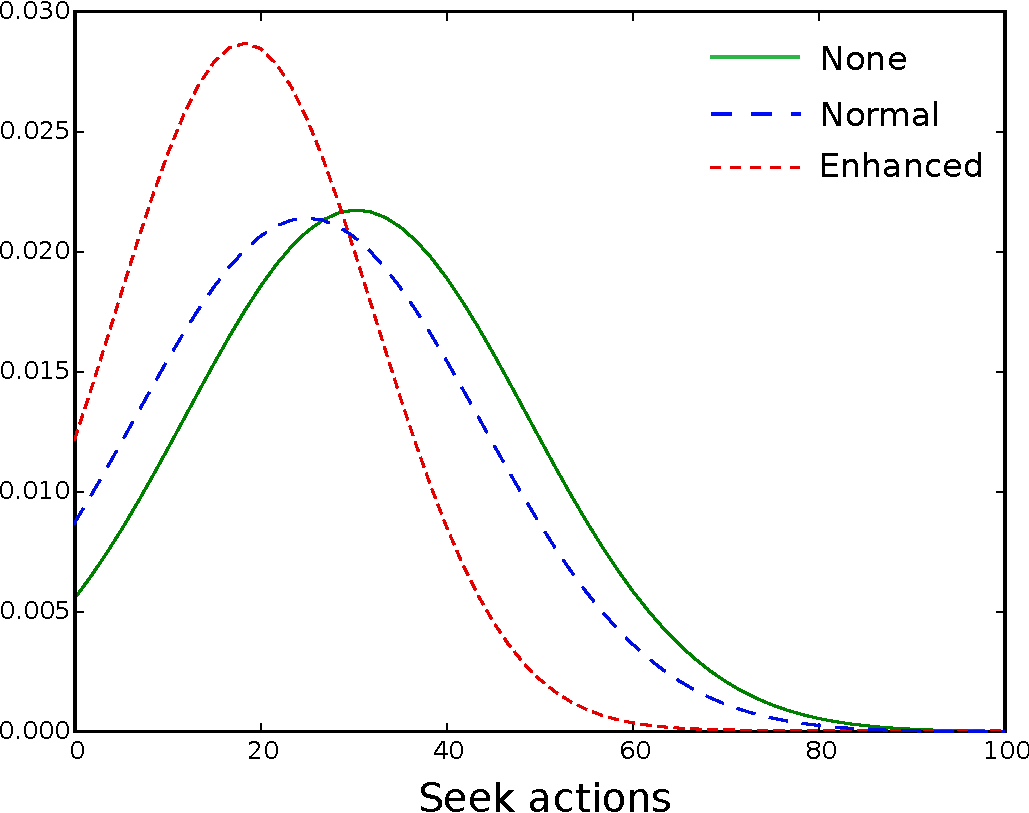
\includegraphics[width=0.6\columnwidth]{figs/seek-pdf.pdf}
%\caption{Probability density function of number of seek actions for each
%visualization}
%\label{fig:seekpdf}
%\end{figure}

%For each metric, the standardisation function (see Equation~\ref{eq:standard}) subtracts the mean of the participant's
%scores and divides by the standard deviation. This maps observations to the `standard score', which is a dimensionless
%unit that represents the number of standard deviations an observation is above the mean.

%\begin{equation}
%std(x) = \frac{x - \mu_{part}}{\highsigma_{part}}
%\label{eq:standard}
%\end{equation}

%The performance and TLX metrics of the 41 accepted participants were analysed using ANOVA.  Significant results were
%found for the number of seek actions ($F_{2,40}=30, p<0.001$) and the selection time ($F_{2,40}=3.2,p\medsig$<0.05$$).  Tukey's
%test shows that the enhanced waveform required fewer seek actions than the normal waveform, and the normal waveform
%required fewer than no waveform (see Figure~\ref{fig:tukeyseekselect}). The selection time was shorter for the enhanced
%waveform compared to no waveform, but the normal waveform was not significantly different.

%\begin{figure}[!h]
%\centering
%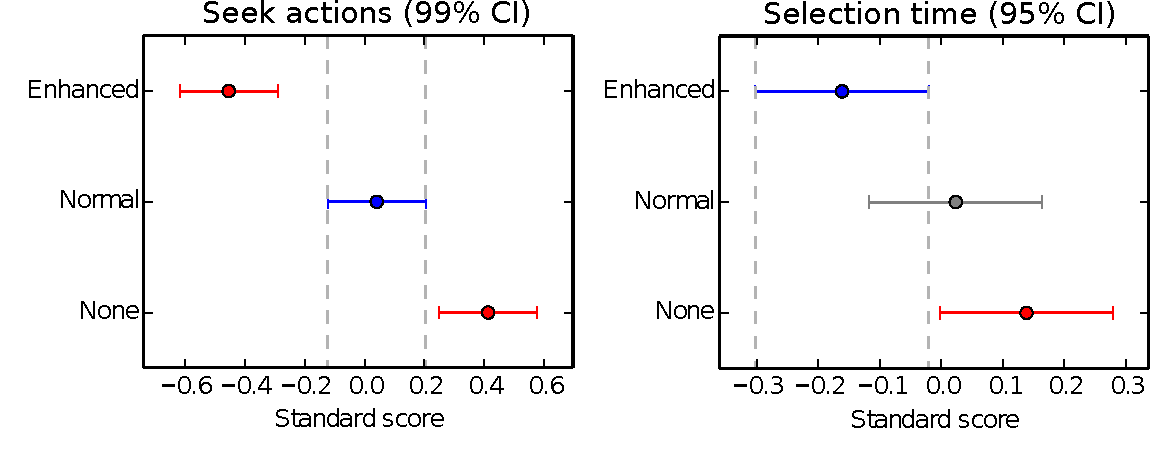
\includegraphics[width=\columnwidth]{figs/seek-select.pdf}
%\caption{Tukey's test for mean number of seek actions and mean selection time}
%\label{fig:tukeyseekselect}
%\end{figure}

%Significant results were found for each of the NASA-TLX metrics ($F_{2,40}>4.8,p\highsig$<0.01$$). The normal waveform performed
%better than no waveform for mental demand, performance, effort and frustration (see Figure~\ref{fig:tlx}). The enhanced
%waveform performed better than the normal waveform for mental, physical and temporal demand, performance and effort.

%\begin{figure}[!h]
%\centering
%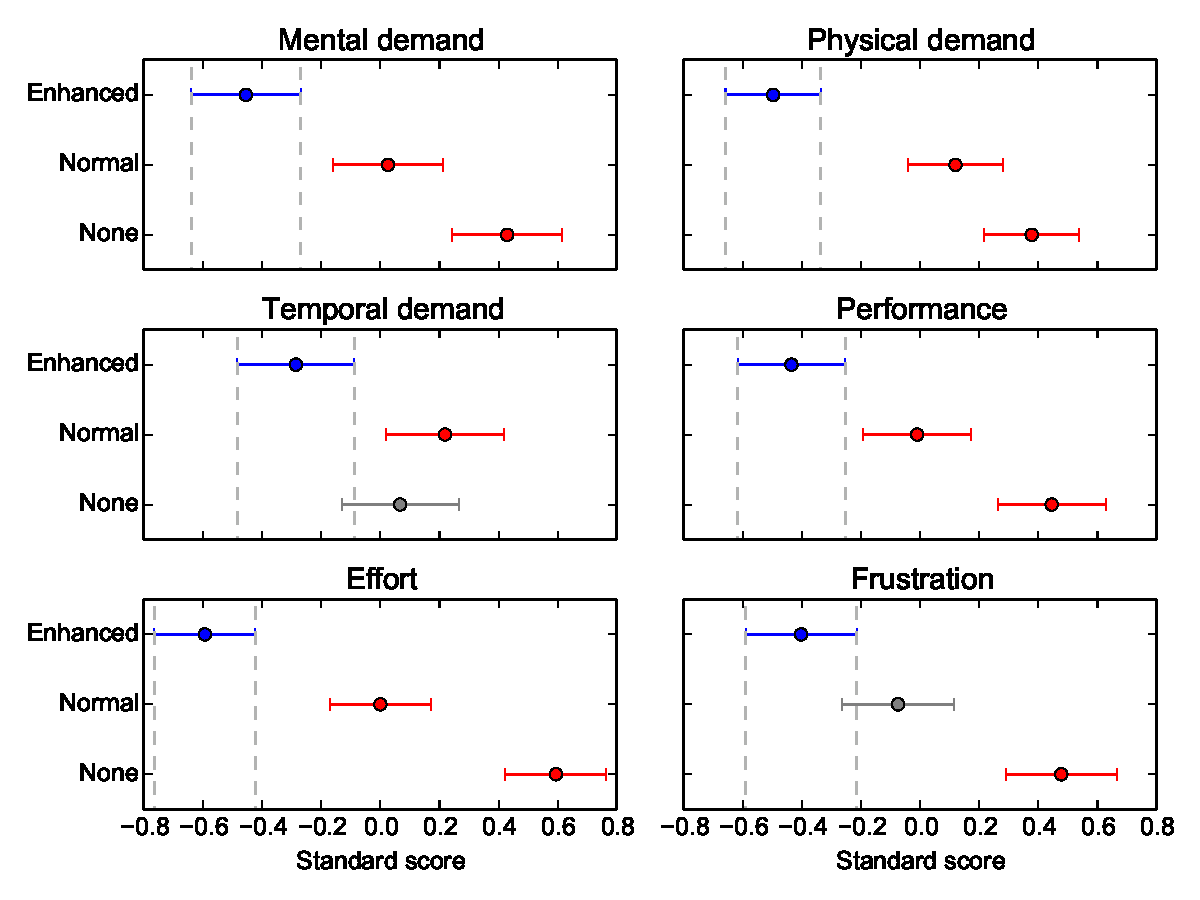
\includegraphics[width=\columnwidth]{figs/tlx-std-tukey95.pdf}
%\caption{Tukey's test for mean of NASA-TLX metrics (95\% CI). Lower is
  %better.}
%\label{fig:tlx}
%\end{figure}

%76\% of participants thought that the enhanced waveform was the easiest to use with the normal waveform scoring 17\%.
%Two-thirds thought that having no waveform was the most frustrating condition with 20\% choosing the normal waveform.

\section{Discussion}\label{sec:vis-discuss}

Our study found that using an enhanced waveform visualization, participants could segment music from speech faster,
more accurately and with less effort than using a normal waveform.  When using the normal waveform, participants could
segment music from speech with less effort than having no visualization, but we did not find any significant
differences in the time it took, nor the accuracy of the result.  Table~\ref{tab:hypotheses} summarises the findings
for the hypotheses we tested.

\begin{table}[h]
  \centering
  \begin{tabular}{l | c c | c c}
    \hline
    & \multicolumn{2}{c|}{Quantitative metrics} & \multicolumn{2}{c}{Qualitative metrics} \\
    \hline
    H1 (effort)   & C1$>$C2 & C2$>$C3 & C1$>$C2 & C2$>$C3 \\
    H2 (time)     & --      & C2$>$C3 & --      & C2$>$C3 \\
    H3 (accuracy) & --      & C2$<$C3 & --      & C2$<$C3 \\
    \hline
  \end{tabular}
  \caption{Summary of confirmed findings for each hypothesis}
  \label{tab:hypotheses}
\end{table}

% enhanced waveforms are better than normal, so what?
% - 30% fewer seek actions
%   - is a lot
%   - don't need to listen as much
%   - better sense of structure
The mean average number of seek actions for the enhanced waveform was 30\% less than for the normal waveform, and the
mean task completion time was 13\% faster. This shows that the participants did not have to navigate the audio as often
to complete the task. This is likely to be because the colour enhancement allowed participants to narrow their search
region, so they did not have to perform as much listening as they otherwise would. The enhanced waveform was also 14\%
more accurate than the normal waveform, potentially because the narrower search region made it easier to find the
precise start and end time of the music.

The increased performance of the enhanced waveform demonstrates that there is potential in the colour mapping
techniques explored by \citet{Tzanetakis2000}, \citet{Rice2005} and \citet{Mason2007}. We did not attempt to select the
best possible semantic audio feature, nor the optimum colour mapping technique, so it is likely that optimising these
would provide much better performance than the visualization we tested.

% - impact on radio production
%   - participants were not professionals, but vast majority had experience of using pro editing software
%   - less experience/training required to get up to performance
%   - would free up more time for creative tasks
Radio programmes must be produced in a limited time period, which means that radio producers often work to tight
deadlines. A reduction in the time and effort needed to perform simple editing tasks could give radio producers greater
freedom to focus on more creative and productive activities. In turn, this could potentially lead to improvements in the
editorial quality of programmes.

% normal are not much better than nothing, so what?
% - waveforms are widely used
%   - impacts on many people
%   - questions over whether waveforms should be default vis
%   - opportunity to make big difference
Although normal waveforms allowed participants to complete our music segmentation task with less effort than no
visualization, there was no significant difference in the task completion time, nor the accuracy of the result.  In a
study made up of 41 participants, we would have expected to find a significant difference compared to the baseline.
This poor performance raises questions over how helpful waveforms are as a navigational aid.

The consequence of poor performance of waveforms is particularly high because waveforms are the default visualization
for most digital audio workstations. With our enhanced waveform, we have seen that it is possible to provide greater
efficiency for navigating and editing audio for at least one task.  Improving the performance of the default
visualizations in DAWs could make a marked difference to a large number of people, as audio editing software is
used around the world by various professionals, many of whom spend much of their working life interacting with audio
using these visualizations.

% - choice of feature
%   - we didn't choose the best
%   - other features may perform better
%   - using multiple features is likely to improve performance further
We selected low energy ratio as a semantic audio feature for discriminating between music and speech.  Low energy ratio
is based on detecting changes in the amplitude profile.  Although these changes can clearly be seen using an audio
waveform, they are only visible when the waveform is sufficiently zoomed-in.  It is therefore important to not only
include the right information, but to present it in a way that humans can read.

We restricted our selection of the semantic audio feature to a one-dimensional value, and used pseudocolour to map the
value to the waveform.  Low energy ratio is just one of many features we could have used for this task.  There are
other features that are more effective and could further improve user performance. Multiple features could
also be combined by using weighting, by using logic to switch between them or by mapping them using false colour.

% applications beyond speech/music discrimination
The ability to visually identify the location of music has applications beyond removal of unwanted music.
\citet{Mason2007} mapped three semantic audio features using false colour to display the structure of radio programmes
to help consumers navigate audio recordings.  Many daytime radio programmes alternate between speech and music, so
being able to see where the music is played would provide a visual structure of the programme. This could help
producers and the audience navigate to the next piece of speech or music, and get a sense of the programme format and
length.

\section{Conclusion}\label{sec:vis-conclusions}

We conducted a within-subjects user study in which 41 participants segmented music from speech using three conditions
-- a normal audio waveform, a waveform enhanced by mapping semantic information to colour, and without using any
visualization.  Based on both quantitative and qualitative metrics, we found that using the enhanced waveform,
participants completed the task faster, more accurately and with less effort than the normal waveform. Using the normal
waveform required less effort than no visualization, but was not significantly faster, nor more accurate.

Our results show that mapping semantic audio features to a visual representation can improve user performance.  Given
the large-scale use of waveforms in audio production, making improvements to the audio visualization could make a
meaningful impact on a large community.  For this study, we selected a rudimentary audio feature and visual mapping.
There are opportunities to develop more efficient audio visualizations by combining multiple features and using more
advanced visualization techniques, targeting either specific applications or general use.

%This experiment used a browser-based audio interface to conduct a within-subjects online study of how users performed
%in finding and selecting music with different audio waveforms. Three conditions were tested -- no waveform, a normal
%waveform and a waveform that was colourised using a simple speech/music discriminator.

%Compared to no waveform, the normal waveform required fewer seek actions and was rated better in terms of mental
%demand, performance, effort and frustration. Finding and selecting music with the colourised version took less time
%than with no waveform. Compared to the normal waveform, it required fewer seek actions and was rated better in terms of
%mental, physical and temporal demand, performance and effort.

%\subsection{Further work}
%The results indicate that the waveform can be significantly improved, even with a simple enhancement. The next stages
%of this research will focus on development of audio analysis and visualization algorithms/tools that address the needs
%of people working in radio production. This will be followed by an analysis of the real-world benefit of using these
%new tools.
